\documentclass[12pt]{book}
\usepackage{amsmath}
\usepackage{amssymb}
\usepackage{amsthm}
\usepackage{amsfonts}
\usepackage{graphicx}
\usepackage{textcomp}
\usepackage{hyperref}
\usepackage{tikz}
\usepackage{enumitem}
\usepackage{mathtools}
\usepackage{enumitem}
\usepackage{wasysym}
\usepackage{ulem}
\usepackage{xspace}
\usepackage{booktabs}
\usepackage{physics}
\usepackage{titlesec}
\usepackage[most]{tcolorbox}

% greenquote and stuff
\newtcolorbox{greenquote}{
  colback=green!20,
  colframe=green!80,
  % fonttitle=\bfseries,
  coltitle=black,
  left=1em,
  right=1em,
  top=0.5em,
  bottom=0.5em,
  boxrule=0.4pt,
  % title={Quote},
  before skip=10pt,
  after skip=10pt,
  sharp corners,
}

\newtcolorbox{redquote}{
  colback=red!20,
  colframe=red!80,
  % fonttitle=\bfseries,
  coltitle=black,
  left=1em,
  right=1em,
  top=0.5em,
  bottom=0.5em,
  boxrule=0.4pt,
  % title={Quote},
  before skip=10pt,
  after skip=10pt,
  sharp corners,
}

\newtcolorbox{yellowquote}{
  colback=yellow!20,
  colframe=yellow!80,
  % fonttitle=\bfseries,
  coltitle=black,
  left=1em,
  right=1em,
  top=0.5em,
  bottom=0.5em,
  boxrule=0.4pt,
  % title={Quote},
  before skip=10pt,
  after skip=10pt,
  sharp corners,
}


\titleformat{\chapter}[display]
  {\normalfont\huge\bfseries}
  {\chaptername\ \thechapter}{20pt}{\Huge}
\titlespacing*{\chapter}{0pt}{0pt}{20pt}

\ifPDFTeX % ensure generation of machine readable output
\input{glyphtounicode}
\pdfgentounicode=1
\usepackage[T1]{fontenc}
\usepackage[utf8]{inputenc}
\usepackage{lmodern}
\fi

\usepackage{csquotes}

\DeclareMathOperator{\dist}{dist}
\DeclareMathOperator{\Nul}{Nul}
\DeclareMathOperator{\Row}{Row}
\DeclareMathOperator{\proj}{proj}

\setlength{\arraycolsep}{12pt}

\newcommand{\Eg}{\textbf{Eg.}\xspace}
\newcommand{\Ex}{\textbf{Ex.}\xspace}
\newcommand{\Ie}{\textbf{I.e.}\xspace}
\newcommand{\bigEps}{\mathcal{E}}
\newcommand{\bproof}{\textit{Proof ($\impliedby$).}\xspace}
\newcommand{\defn}{\textbf{Def.}\xspace}
\newcommand{\eg}{\textbf{e.g.}\xspace}
\newcommand{\ex}{\textbf{ex.}\xspace}
\newcommand{\fproof}{\textit{Proof ($\implies$).}\xspace}
\newcommand{\ie}{\textbf{i.e.}\xspace}
\newcommand{\lemma}{\textit{Lemma}\xspace}
\newcommand{\soln}{\textit{Soln.}\xspace}
\newcommand{\thm}{\textbf{Thm.}\xspace}
\newcommand{\fl}{\operatorname{fl}}

\renewcommand{\arraystretch}{1.25} % Adjust row spacing

\hypersetup{
    colorlinks=true,
    linkcolor=blue,
    filecolor=blue,      
    urlcolor=blue,
}

\newcommand{\ulhref}[2]{\href{#1}{\color{blue}\uline{#2}}}

\begin{document}

\title{Numerical Analysis: The Definitive Edition}
\author{Alexander Ng}
\date{Monday, April 14, 2025\\\small Last Updated: \today}

\maketitle
\section*{Foreword}

Hi reader, the following is a collection of notes I took while taking SFU's MACM
316 (Numerical Analysis) in Spring 2025. Many of the notes are heavily based on
the lecture notes given by Professor Steven Ruuth, which can be found in this
repository at \texttt{./steve's notes}. I have tried to make the notes as
readable as possible, and every file is compiled in a machine-readable format so
you can easily stick them into an AI knowledge base to help you with your
studies.

If you need help getting back up to speed on Linear Algebra, I highly recommend
taking a look at \ulhref{https://venhance.github.io/napkin/Napkin.pdf#part.4}{An Infinitely Large Napkin} by Venhance. It's a great book that covers all of the
theory of mathematics that you will need to understand the material in this
course.
Overtime, I will be updating these notes to be better structured based on the
chapters of the textbook that the course is structured around.

\tableofcontents
\clearpage

\chapter{An Introduction to Numerical Analysis}
\begin{greenquote}
  The first four lectures of this course are an introduction to numerical
  analysis and the main recurring concepts that will be used throughout the
  course.
\end{greenquote}
Many real-world problems stem from numerical analysis, particularly poor 
execution. Rounding errors, insufficient representation problems, and other 
such problems represent the significant impact of computation in the real world.

Check out the following resources for more information:
\begin{enumerate}
  \item \ulhref{https://www-users.cse.umn.edu/~arnold/disasters/}{https://www-users.cse.umn.edu/~arnold/disasters/}
  \item \ulhref{https://web.ma.utexas.edu/users/arbogast/misc/disasters.html}{https://web.ma.utexas.edu/users/arbogast/misc/disasters.html}
\end{enumerate}

\section{Computer Arithmetic}
\begin{greenquote}
  In Spring 2025, this was the start of Lecture 1.
\end{greenquote}

We often want to work with the real number system, which consists of all 
integers, rational and irrational numbers
\begin{equation*}
  2, \sqrt{2}, e, \pi, 10^6, \text{ etc.} 
\end{equation*}
Because we have a finite space limitation for numbers, 
\textbf{not all numbers can be represented exactly.} This can cause problems
with arithmetic.

\subsection{Bases - Binary and Decimal}

We typically use the decimal (base 10) system, e.g.
\begin{equation*}
  427.325 = 4 \times 10^2 + 2 \times 10^1 + 7 \times 10^{0} + 3 \times 10^{-1}+\dots
\end{equation*}
However, when we work with a computer, we use the binary (base 2) system:
\begin{equation*}
  (1001.11101)_2 = 1\times 2^3 + 0\times 2^2 + 0\times 2 + 1\times 2^0 + 1\times 2^{-1} + 1\times 2^{-2} + 1\times 2^{-3} +\dots
\end{equation*}
In this class, we will only be working in the decimal system in order to make
computations simpler, since the application of concepts is identical.

\subsection{Base Conversion and Error}

Because it is impossible to represent some finite decimal fractions in binary,
we will (definitely) encounter \textbf{error} when converting from base-10 to
base-2. In the following example, we will convert $\frac{1}{10}$ to binary, and
show how there exists some numbers which cannot be represented exactly within 
the binary floating-point system.

% Notice that conversion from base-10 to base-2 can lead to errors. It is 
% impossible to represent some finite decimal fractions in binary.

\subsubsection{Example}

To convert a decimal fraction like $\frac{1}{10}$ into its binary 
representation, we repeatedly multiply the fractional part by $2$ and extract
the integer part at each step.

We begin with $1/10 = 0.1_{10}$, and assume $0.1_{10} = (a_1.a_2a_3\dots
a_n)_2$.
\[
\frac{1}{10} = 0.1_{10} = (0.a_1a_2a_3\dots a_n)_{2}
\]

Multiply by $2$:
\[
2 \times 0.1 = 0.2 = (a_1.a_2a_3\dots)_2
\]

Keep the fractional part and repeat:
\begin{align*}
  &a_1 = \lfloor 0.2 \rfloor = 0 \\
  2 \times 0.2 = 0.4 \implies &a_2 = \lfloor 0.4 \rfloor = 0 \\
  2 \times 0.4 = 0.8 \implies &a_3 = \lfloor 0.8 \rfloor = 0 \\
  2 \times 0.8 = 1.6 \implies &a_4 = \lfloor 1.6 \rfloor = 1 \\
  1.6 - 1 &= 0.6 \\
  2 \times 0.6 = 1.2 \implies &a_5 = \lfloor 1.2 \rfloor = 1 \\
  1.2 - 1 &= 0.2
\end{align*}

We have now returned to $0.2$, which was the value after the very first 
multiplication. This means the process will repeat indefinitely. Thus, the 
binary representation of $\frac{1}{10}$ is:
\[
  \frac{1}{10} = (0.0\mathbf{0011}00110011\dots)_2
\]
The repeating part is \textbf{0011}\dots, and this pattern continues forever. 
Using a finite number of digits, $\frac{1}{10}$ \textbf{cannot} be represented
exactly in binary. Just as $\frac{1}{3} = 0.\overline{3}$ cannot
be perfectly represented in decimal, the same is true for $\frac{1}{10}$ in
binary. This is why certain decimal fractions lead to rounding errors in binary-
based floating-point arithmetic.

\section{Hypothetical Storage Scheme (32-bit)}

We will use a hypothetical decimal computer since the concept is identical.
(By the way, this is very close to 
\ulhref{https://en.wikipedia.org/wiki/IEEE_754}{IEEE-754} floating point
representation, except that we are using a decimal representation instead of
binary.)

Suppose we have the decimal number $423.7$. Since we always want to represent
numbers in proper scientific notation, we normalize the
\textbf{mantissa}.
We write our number as follows:

\begin{equation*}
  423.7 = +\underbrace{0.4237}_{\text{mantissa}} \times 10^{+3}
\end{equation*}
Notice the $+$ is relevant because we require an explicit representation of the
sign of the number. We call the bits following from the decimal point ($4273$) 
the \textbf{mantissa}.
We include 1 bit for the sign, which is $1$ for positive numbers, 1 bit for the
exponent sign, 7 bits for the exponent, and the remaining 23 bits for the
mantissa.

\begin{figure}[h]
  \centering
  \includegraphics[width=0.8\textwidth]{./assets/fake_ieee754.png}
  \caption{Hypothetical Storage Scheme (32-bit)}
\end{figure}

\subsection{Problems with Floating Point}
\noindent
\begin{minipage}{\textwidth}
Because our storage format is finite, the biggest problems we will encounter
are:
\begin{enumerate}
  \item \textbf{bit overflow}: the maximum magnitude of our exponent (in binary)
    is \textbf{127}, so our number can only range from $2^{-127}$ to $2^{+127}$.
  \item \textbf{rounding error}: because our mantissa only has 23 bits of 
    precision, the precision will decrease as our numbers get larger because we 
    use exponentiation to represent the actual number.
\end{enumerate}
\end{minipage}

% Because our storage format is finite, one of the biggest problems we will 
% encounter is \textbf{bit overflow}. The maximum magnitude of our exponent 
% (in binary) is \textbf{127}, so our number can only range from $2^{-127}$ to
% $2^{+127}$. Because our mantissa only has 23 bits of precision, the precision
% will decrease as our numbers get larger because we use exponentiation to 
% represent the actual number.

\subsubsection{Error Example}

Consider the number $2^{25} = 33,554,432$. This number can be represented 
exactly in binary. However, the number $2^{25}+1 = 33,554,433$ cannot be
represented exactly, since it can't fit within the 23 bits of precision available.

From this, we find that all numbers (including fractions) from $2^{25}-1$ 
through $2^{25}+2$ are represented with the same mantissa in binary. Only when 
you reach $2^{25}+3$ does the mantissa change.

\subsubsection{Remarks}

Within IEEE-754-style floating point representation, the
number of representable values within a given exponent is the same, regardless
of the exponent. This may seem obvious, but it's interesting nonetheless. This
comes from the fact that the number of bits in the mantissa is fixed. The
number of representable values is exactly $2\times 2^{23} = 2^{24}$, since each
positive value has a negative counterpart.

\subsubsection{Actual IEEE-754 Floating Point}
There are a few key differences betewen our hypothetical storage scheme and the
actual IEEE-754 specification.

\begin{enumerate}
  \item Instead of an exponent sign bit, IEEE-754 specifies a \textbf{biased
    exponent} which just stores the exponent as an 8-bit unsigned integer and
    interprets it as $2^{e-127}$. \Ex we want $2^{2}$ to be the exponent part of
    our number, so we set the biased exponent to $e=2+127=129$. When we decode
    the number, we multiply the mantissa by $2^{129-127 = 2}$ to get the actual
    number.
  \item The hidden bit (implicit leading 1) is a feature of IEEE-754 that allows
    us to \enquote{fake} 24 bits of mantissa precision. We save a bit by
    specifying the zeroth bit of the mantissa as always being a 1, and we can
    use this fact to save one bit of space.
\end{enumerate}
In IEEE-754, the number is represented as
\[
  (-1)^{s} \times 1.f \times 2^{e-127}
.\]
where $s$ is the sign bit, $f$ is the mantissa, and $e$ is the biased exponent.

\newpage
\section{Floating Point Decimal Normalization}
\begin{greenquote}
  In Spring 2025, this was the start of Lecture 2.
\end{greenquote}

Can we write all real numbers in normalized scientific notation? Well, the short
answer is yes.
\begin{align*}
    732.5051 &\rightarrow +0.7325051 \times 10^{+3} \\
    -0.005612 &\rightarrow -0.5612 \times 10^{-2}
\end{align*}
For $x \in \mathbb{R}$, we can express it as:
\begin{equation*}
    x = \pm r \times 10^{\pm n}, \quad \text{where } \frac{1}{10} \leq r \leq 1.
\end{equation*}
In binary, we write:
\begin{equation*}
  x = \pm q \times 2^{\pm m}, \quad \text{where } \frac{1}{2} \leq q < 1.
\end{equation*}
Here, $q$ is the mantissa and $m$ is the integer exponent.

Let $b$ be the base.
We limit $r$ and $q$ because when $k < 1/b$, we can shift the decimal 
place and normalize the number further. When we have $1.d_1$, we rewrite it 
as $0.1d_1 \times b^1$.

\section{What if we have too many digits?}
Oftentimes, we will be doing computations with a finite number of digits, but
using operations that increase the number of digits. For example, if we multiply 
$\frac{1}{8} = 0.125$ (3 significant digits) by $\frac{1}{7} = 0.142857$ (5
significant digits) we get $0.017857125$ (8 significant digits). This is
a problem, since at a certain point, we will have too many digits to represent
the number accurately. To solve this problem, we have rounding and truncation.

\subsection{Rounding}
% \section{Rounding and Chopping}
 % (Sources of Error)
Given $x = 0.a_1 a_2 \dots a_n a_{n+1} \dots a_m$ using $m$ digits, rounding 
to $n$ places follows:
\begin{itemize}
  \item If $0 \leq a_{n+1} < 5$, then $x = 0.a_1 a_2 \dots a_n$.
  \item If $5 \leq a_{n+1} \leq 9$, then $x = 0.a_1 a_2 \dots (a_n + 1)$.
\end{itemize}
As you will see in the following example, this definition of rounding is
different from the way we traditionally round numbers. We only consider the
magnitude of the smallest significant digit, not the sign, so that when you
round a number and its additive inverse, they will still cancel out.

\subsubsection{Example}
\begin{align*}
  \text{round}(0.125) &= 0.13, \\
  \text{round}(-0.125) &= -0.13.
\end{align*}

Suppose, instead, that we define rounding classically, where we round to the
nearest digit. Then, we would round $0.125$ to $0.12$ and $-0.125$ to $-0.13$,
and adding $0.125+ (-0.125) = 0$ would result in $0.12 + (-0.13) = -0.01$, which
is definitely wrong.

\subsection{Chopping (Truncation)}
Compared to rounding, truncation/chopping to $n$ decimal places follows:
\begin{align*}
  x &= 0.a_1 a_2 \dots a_na_{n+1} \dots a_m, \\
  \text{chop}_n(x) &= 0.a_1 a_2 \dots a_n.
\end{align*}

Truncation introduces larger errors but is computationally cheaper than 
rounding. In general, we prefer rounding because of the higher accuracy, because
the computational cost is generally considered negligible.

\section{Error}

Because this class is called Numerical \textbf{Analysis}, we care a lot about
the accuracy of our computations, and therefore we need to be able to quantify
the error of the methods we use. Make sure to memorize the following
definitions, especially if your professor does not allow you to have a formula
sheet on the midterm(s)/final exam.

\subsection{Definitions}

\begin{minipage}{\textwidth}
  \begin{itemize}
    \item Actual error: $p - \hat{p}$. Use case: when the direction of the error
      matters (e.g. bias detection, error cancellation).
    \item Absolute error: $\abs{p - \hat{p}}$. Use case: you only care about the
      magnitude of the error (e.g. reporting precision).
    \item Relative error: $\frac{\abs{p - \hat{p}}}{\abs{p}}$. Use case: we need
      a scale-independent measure of error (\ie how big is the error relative to
      the magnitude of the value).
  \end{itemize}
  \small *The notes use $p$ and $p^*$ but I will use them interchangeably with
  $p$ and $\hat{p}$.
\end{minipage}

\subsection{Significant Digits}
An approximation $\hat p$ has $t$ significant digits if

\begin{equation*}
  \frac{\abs{p-\hat p}}{\abs{p}} \leq 5 \times 10^{-t}. 
\end{equation*}
we call $5\times 10^{-t}$ the \textbf{error bound}.

\subsection{Example}

Our exact value is $0.1$ and we approximate it with $0.099$. The relative error
is:
\[
  \frac{\abs{0.1 - 0.099}}{\abs{0.1}} = 0.01
.\]

\begin{center}
  \begin{tabular}{c|c|c}
    $t$ & $5 \times 10^{-t}$ & error $\leq$ bound? \\
    \hline
    0 & 5 & $\checkmark$ \\
    1 & 0.5 & $\checkmark$ \\
    2 & 0.05 & $\checkmark$ \\
    3 & 0.005 & $\times$ \\
  \end{tabular}
\end{center}
Since $0.01 < 5 \times 10^{-2}$ but not $5 \times 10^{-3}$, we have two 
significant digits.

\section{Computations and Machine Representation}

Let $\fl(x)$ denote the machine representation of $x$. Computations on a 
machine follow:
\begin{equation*}
    \fl(\fl(x) + \fl(y)).
\end{equation*}
Each step introduces an error.

\subsection{Example}
\begin{align*}
    p &= 0.54617, \quad q = 0.54601, \\
    r &= p - q = 0.00016.
\end{align*}
With 4-digit rounding,
\begin{align*}
  \hat{p} &= 0.5462, \quad \hat{q} = 0.5460, \\
  \hat{r} &= \hat{p} - \hat{q} = -0.0002.
\end{align*}
Relative error:
\begin{equation*}
  \frac{|r - \hat{r}|}{|r|} = 0.25.
\end{equation*}
A high relative error results when subtracting close numbers.

% possibly rewrite this section because it introduces two concepts at once
\section{Roundoff Error} % continued into Lecture 003

Consider computing $\displaystyle f(x) = \frac{1 - \cos x}{x^2}$ for $\bar{x} = 1.2 \times 10^{-5}$.
With 10-digit rounding:
\begin{align*}
    c &= \fl(\cos \bar{x}) = 0.9999999999, \\
    1 - c &= 0.0000000001.
\end{align*}
In this case, the roundoff error causes a \textbf{catastrophic
cancellation}, which 
results in a large error.
Instead, if we use an alternative formula, such as $\cos x = 1 - 2\sin^2(x/2)$:
\begin{equation*}
    f(x) = \frac{1}{2} \left( \frac{\sin(x/2)}{x/2} \right)^2,
\end{equation*}
We obtain a more accurate computation.

% possibly remove this part
\textbf{Conclusion:} Avoid subtracting close numbers. Use alternative 
representations like Taylor series, trigonometric identities or rationalized 
approximations.

\subsection{Reducing Roundoff Error}
\begin{greenquote}
  In Spring 2025, this was the start of Lecture 3.
\end{greenquote}

One way to reduce roundoff error is to minimize the number of floating-point 
operations.

\subsubsection{Polynomial Evaluation Using Nested Multiplication}

Consider evaluating the polynomial:
\begin{equation*}
    f(z) = 1.01z^4 - 4.62z^3 - 3.11z^2 + 12.2z - 1.99.
\end{equation*}
We can rewrite this expression using nested multiplication:
\begin{align*}
    f(z) &= (1.01z^3 - 4.62z^2 - 3.11z + 12.2)z - 1.99 \\
         &= ((1.01z^2 - 4.62z - 3.11)z + 12.2)z - 1.99 \\
         &= \pqty{
           \pqty{
             \pqty{
               1.0z - 4.62
             }z - 3.11
           }z + 12.2
         }z - 1.99 \\
\end{align*}
By factoring out $z$ as much as possible, we reduce the total number of 
floating-point operations, minimizing roundoff error accumulation.

\section{Cancellation Errors}
Otherwise known as catastrophic cancellation.

\subsection{Quadratic Formula and Cancellation Errors}

Consider solving the quadratic equation:
\begin{equation*}
    ax^2 + bx + c = 0.
\end{equation*}
Using the quadratic formula, the roots are:
\begin{align*}
    &x_1 = \frac{-b + \sqrt{b^2 - 4ac}}{2a}
    &x_2 = \frac{-b - \sqrt{b^2 - 4ac}}{2a}.
\end{align*}
Suppose $b = 600$, $a = c = 1$. Then we have
\begin{align*}
  &x_1 = \frac{-600 + \sqrt{600^2 - 4 \cdot 1 \cdot 1}}{2 \cdot 1}, \quad
  &x_2 = \frac{-600 - \sqrt{600^2 - 4 \cdot 1 \cdot 1}}{2 \cdot 1} \\
  &x_1 = \frac{-600 + \sqrt{359996}}{2}, 
  &x_2 = \frac{-600 - \sqrt{359996}}{2}
\end{align*}

You'll notice that $\sqrt{359996} = 599.9966666574$ is very close to $600$. This
is a pretty big problem.

Since $b$ is large and $a, c$ are small, the term $\sqrt{b^2 - 4ac}$
is very close to $b$. This causes \textbf{catastrophic cancellation} in the
computation of $x_1$, where subtracting two nearly equal quantities leads to
significant loss of precision in floating-point arithmetic.

% The issue arises because $-b$ is close in 
% magnitude to $+\sqrt{b^2 - 4ac}$, causing significant cancellation error in 
% $x_1$.

\subsection{Reformulating to Reduce Cancellation}

We rationalize the numerator:
\begin{equation*}
    x_1 = \frac{(-b + \sqrt{b^2 - 4ac})}{2a} \times 
          \frac{(-b - \sqrt{b^2 - 4ac})}{(-b - \sqrt{b^2 - 4ac})}.
\end{equation*}

This simplifies to:
\begin{equation*}
    x_1 = \frac{b^2 - (b^2 - 4ac)}{2a(-b - \sqrt{b^2 - 4ac})} = 
    \frac{2c}{-b - \sqrt{b^2 - 4ac}}.
\end{equation*}
Now, the cancellation error is eliminated. If, suppose, $b = -600$, the same 
issue would occur with $x_2$, and we could apply the same rationalization
technique.

\tiny You should write this down on your cheat sheet.\normalsize

% maybe new page
\section{Review of Taylor Series}

Taylor’s theorem is fundamental for numerical approximations.

\subsection{Definition of Taylor Series}

\begin{minipage}{\textwidth}
Given a function $f(x)$ that is sufficiently smooth on $[a, b]$, we can 
approximate $f(x)$ with a Taylor polynomial $P_n(x)$:
\begin{equation*}
    P_n(x) = f(x_0) + f'(x_0)(x - x_0) + \frac{f''(x_0)}{2!} (x - x_0)^2 + 
             \dots + \frac{f^{(n)}(x_0)}{n!} (x - x_0)^n.
\end{equation*}
Here, $x_0, x \in [a, b]$.
\end{minipage}

\subsection{Conditions for Taylor Series Expansion}

For $f(x)$ to have a valid Taylor series expansion:
\begin{itemize}
  \item $f \in C^n[a, b]$
    \begin{itemize}
      \item This reads \enquote{f is continuous to the $n$th derivative on the
        interval $[a, b]$}.
        \tiny *Remember this\normalsize
      \item \ie $f$, $f'$, $f''$, ..., $f^n$ must be continuous
    \end{itemize}
  \item $f^{(n+1)}$ must exist on $[a, b]$.
\end{itemize}

\subsection{Error in Taylor Approximation}

The error in a Taylor series approximation is given by:
\begin{equation*}
    f(x) = P_n(x) + R_n(x),
\end{equation*}
where the remainder term $R_n(x)$ satisfies:
\begin{equation*}
    R_n(x) = \frac{f^{(n+1)}(c)}{(n+1)!} (x - x_0)^{n+1},
\end{equation*}
for some $c \in (x_0, x)$. The approximation is most accurate when $x$ is 
close to $x_0$.

\subsection{Example: Third-Order Taylor Polynomial}

Find $P_3(x)$ for $f(x) = \sin(x)$ centered at $x_0 = 0$.
\begin{align*}
    P_3(x) &= f(0) + f'(0)(x - 0) + \frac{f''(0)}{2!} (x - 0)^2 + 
             \frac{f'''(0)}{3!} (x - 0)^3 \\
           &= x - \frac{x^3}{6}.
\end{align*}

\subsubsection{Error Analysis}
The remainder term for $n = 3$ is:
\begin{equation*}
    R_3(x) = \frac{f^{(4)}(c)}{4!} x^4.
\end{equation*}
substituting $f^{(4)}(x) = \sin(x)$,
\begin{equation*}
    R_3(x) = \frac{\sin(c)}{24} x^4.
\end{equation*}
and finally, taking $x = 0.1$:
\begin{equation*}
    |R_3(0.1)| \leq \frac{|\sin(0.1)|}{24} (0.1)^4 < 4.2 \times 10^{-7}.
\end{equation*}
A $10^{-7}$ relative error is more than enough to be considered high accuracy.

\subsection{Example: Linear Approximation of $\sqrt{16.1}$}
\begin{greenquote}
  In Spring 2025, this was the start of Lecture 2.
\end{greenquote}

We use $P_1$ (linear approximation) to find an approximation of $\sqrt{16.1}$
without using the square root algorithm.

\subsubsection{Solution}
Let $f(x) = \sqrt{x}$ and choose an expansion point $x_0 = 16$, since 
$\sqrt{16} = 4 \in \mathbb{Z}$ is easily computable. Using the first-order 
Taylor approximation:
\begin{equation*}
    f(x_0 + h) \approx f(x_0) + h f'(x_0),
\end{equation*}
where $h = 0.1$.

\subsubsection{Computation}
\begin{align*}
    f(16) &= \sqrt{16} = 4, \\
    f'(x) &= \frac{1}{2\sqrt{x}}, \quad f'(16) = \frac{1}{8}, \\
    f(16.1) &\approx 4 + 0.1 \times \frac{1}{8} = 4.0125.
\end{align*}
The exact value is $4.01248052955\dots$, with a small truncation error.
Since the machine error is on the order of $10^{-14}$, it is negligible compared 
to the Taylor approximation error.

\section{Algorithm Quantification}

Numerical methods construct a sequence of better and better approximations, 
converging to a solution $\alpha$.

Given a sequence $\{\alpha_n\}$:
\begin{equation*}
    \lim_{n\to\infty} \alpha_n = \alpha.
\end{equation*}
We quantify convergence speed by analyzing $|\alpha - \alpha_n| \leq c$, where 
$c$ is a target error.

\subsection{Example: Convergence of $\sin(1/n)$}

Consider $\alpha_n = \sin(1/n)$, which converges to $\alpha = 0$ as $n \to \infty$.
We rewrite:
\begin{equation*}
    \lim_{n \to \infty} \sin(1/n) = \lim_{h \to 0} \sin(h),
\end{equation*}
which is easier to analyze. Expanding $\sin(h)$ in a Taylor series:
\begin{equation*}
    \sin(h) = h - \frac{h^3}{3!} + \frac{h^5}{5!} + \dots.
\end{equation*}
For small $h$, $\sin(h) \approx h$, implying:
\begin{equation*}
    |\alpha_n - \alpha| \leq \frac{1}{n}.
\end{equation*}
Thus, $\alpha_n$ converges to $\alpha = 0$ with rate of convergence $O(1/n)$.

\section{Big-O Notation}

For a sequence $\{A_n\}$, if:
\begin{equation*}
    |A_n - A| \leq k |B_n| \quad \text{for sufficiently large } n,
\end{equation*}
where $k$ is a constant, then we say:
\begin{equation*}
    A_n = A + O(B_n).
\end{equation*}

\subsection{Example: $\sin(1/n)$ Convergence}

From before, $|\alpha_n - \alpha| \leq 1/n$, so:
\begin{equation*}
    A_n = \sin(1/n) \text{ converges to } A = 0 
    \text{ with rate of convergence } O(1/n).
\end{equation*}

\subsection{Example: Convergence of $n \sin(1/n)$}

We evaluate:
\begin{equation*}
    \lim_{n \to \infty} n \sin(1/n) = 1.
\end{equation*}
Changing variables, $h = 1/n$, we obtain:
\begin{equation*}
    \lim_{h \to 0} \frac{\sin(h)}{h} = 1.
\end{equation*}
Expanding $\sin(h)/h$ in Taylor form:
\begin{equation*}
    \frac{\sin(h)}{h} = 1 - \frac{h^2}{6} + O(h^4).
\end{equation*}
For small $h$:
\begin{equation*}
    \frac{\sin(h)}{h} - 1 \approx -\frac{h^2}{6},
\end{equation*}
so $\alpha_n$ converges to $\alpha = 1$ with rate $O(1/n^2)$.

\subsection{Takeaways}

Big-O notation quantifies algorithm efficiency by ignoring constants and focusing 
on convergence trends. Constants vary across systems, so we care about general 
convergence patterns rather than specific values.

% \section{Computer Arithmetic}

We often want to work with the real number system, which consists of all 
integers, rational and irrational numbers
\begin{equation*}
  2, \sqrt{2}, e, \pi, 10^6, \text{ etc.} 
\end{equation*}
Because we have a finite space limitation for numbers, 
\textbf{not all numbers can be represented exactly.} This can cause problems
with arithmetic.

\subsection{Bases - Binary and Decimal}

We typically use the decimal (base 10) system, e.g.
\begin{equation*}
  427.325 = 4 \times 10^2 + 2 \times 10^1 + 7 \times 10^{0} + 3 \times 10^{-1}+\dots
\end{equation*}
However, when we work with a computer, we use the binary (base 2) system:
\begin{equation*}
  (1001.11101)_2 = 1\times 2^3 + 0\times 2^2 + 0\times 2 + 1\times 2^0 + 1\times 2^{-1} + 1\times 2^{-2} + 1\times 2^{-3} +\dots
\end{equation*}
In this class, we will only be working in the decimal system in order to make
computations simpler, since the application of concepts is identical.

\subsection{Base Conversion and Error}

Because it is impossible to represent some finite decimal fractions in binary,
we will (definitely) encounter \textbf{error} when converting from base-10 to
base-2. In the following example, we will convert $\frac{1}{10}$ to binary, and
show how there exists some numbers which cannot be represented exactly within 
the binary floating-point system.

% Notice that conversion from base-10 to base-2 can lead to errors. It is 
% impossible to represent some finite decimal fractions in binary.

\subsubsection{Example}

To convert a decimal fraction like $\frac{1}{10}$ into its binary 
representation, we repeatedly multiply the fractional part by $2$ and extract
the integer part at each step.

We begin with $1/10 = 0.1_{10}$, and assume $0.1_{10} = (a_1.a_2a_3\dots
a_n)_2$.
\[
\frac{1}{10} = 0.1_{10} = (0.a_1a_2a_3\dots a_n)_{2}
\]

Multiply by $2$:
\[
2 \times 0.1 = 0.2 = (a_1.a_2a_3\dots)_2
\]

Keep the fractional part and repeat:
\begin{align*}
  &a_1 = \lfloor 0.2 \rfloor = 0 \\
  2 \times 0.2 = 0.4 \implies &a_2 = \lfloor 0.4 \rfloor = 0 \\
  2 \times 0.4 = 0.8 \implies &a_3 = \lfloor 0.8 \rfloor = 0 \\
  2 \times 0.8 = 1.6 \implies &a_4 = \lfloor 1.6 \rfloor = 1 \\
  1.6 - 1 &= 0.6 \\
  2 \times 0.6 = 1.2 \implies &a_5 = \lfloor 1.2 \rfloor = 1 \\
  1.2 - 1 &= 0.2
\end{align*}

We have now returned to $0.2$, which was the value after the very first 
multiplication. This means the process will repeat indefinitely. Thus, the 
binary representation of $\frac{1}{10}$ is:
\[
  \frac{1}{10} = (0.0\mathbf{0011}00110011\dots)_2
\]
The repeating part is \textbf{0011}\dots, and this pattern continues forever. 
Using a finite number of digits, $\frac{1}{10}$ \textbf{cannot} be represented
exactly in binary. Just as $\frac{1}{3} = 0.\overline{3}$ cannot
be perfectly represented in decimal, the same is true for $\frac{1}{10}$ in
binary. This is why certain decimal fractions lead to rounding errors in binary-
based floating-point arithmetic.

\section{Hypothetical Storage Scheme (32-bit)}

We will use a hypothetical decimal computer since the concept is identical.
(By the way, this is very close to 
\ulhref{https://en.wikipedia.org/wiki/IEEE_754}{IEEE-754} floating point
representation, except that we are using a decimal representation instead of
binary.)

Suppose we have the decimal number $423.7$. Since we always want to represent
numbers in proper scientific notation, we normalize the
\textbf{mantissa}.
We write our number as follows:

\begin{equation*}
  423.7 = +\underbrace{0.4237}_{\text{mantissa}} \times 10^{+3}
\end{equation*}
Notice the $+$ is relevant because we require an explicit representation of the
sign of the number. We call the bits following from the decimal point ($4273$) 
the \textbf{mantissa}.
We include 1 bit for the sign, which is $1$ for positive numbers, 1 bit for the
exponent sign, 7 bits for the exponent, and the remaining 23 bits for the
mantissa.

\begin{figure}[h]
  \centering
  \includegraphics[width=0.8\textwidth]{./assets/fake_ieee754.png}
  \caption{Hypothetical Storage Scheme (32-bit)}
\end{figure}

\subsection{Problems with Floating Point}
\noindent
\begin{minipage}{\textwidth}
Because our storage format is finite, the biggest problems we will encounter
are:
\begin{enumerate}
  \item \textbf{bit overflow}: the maximum magnitude of our exponent (in binary)
    is \textbf{127}, so our number can only range from $2^{-127}$ to $2^{+127}$.
  \item \textbf{rounding error}: because our mantissa only has 23 bits of 
    precision, the precision will decrease as our numbers get larger because we 
    use exponentiation to represent the actual number.
\end{enumerate}
\end{minipage}

% Because our storage format is finite, one of the biggest problems we will 
% encounter is \textbf{bit overflow}. The maximum magnitude of our exponent 
% (in binary) is \textbf{127}, so our number can only range from $2^{-127}$ to
% $2^{+127}$. Because our mantissa only has 23 bits of precision, the precision
% will decrease as our numbers get larger because we use exponentiation to 
% represent the actual number.

\subsubsection{Error Example}

Consider the number $2^{25} = 33,554,432$. This number can be represented 
exactly in binary. However, the number $2^{25}+1 = 33,554,433$ cannot be
represented exactly, since it can't fit within the 23 bits of precision available.

From this, we find that all numbers (including fractions) from $2^{25}-1$ 
through $2^{25}+2$ are represented with the same mantissa in binary. Only when 
you reach $2^{25}+3$ does the mantissa change.

\subsubsection{Remarks}

Within IEEE-754-style floating point representation, the
number of representable values within a given exponent is the same, regardless
of the exponent. This may seem obvious, but it's interesting nonetheless. This
comes from the fact that the number of bits in the mantissa is fixed. The
number of representable values is exactly $2\times 2^{23} = 2^{24}$, since each
positive value has a negative counterpart.

\subsubsection{Actual IEEE-754 Floating Point}
There are a few key differences betewen our hypothetical storage scheme and the
actual IEEE-754 specification.

\begin{enumerate}
  \item Instead of an exponent sign bit, IEEE-754 specifies a \textbf{biased
    exponent} which just stores the exponent as an 8-bit unsigned integer and
    interprets it as $2^{e-127}$. \Ex we want $2^{2}$ to be the exponent part of
    our number, so we set the biased exponent to $e=2+127=129$. When we decode
    the number, we multiply the mantissa by $2^{129-127 = 2}$ to get the actual
    number.
  \item The hidden bit (implicit leading 1) is a feature of IEEE-754 that allows
    us to \enquote{fake} 24 bits of mantissa precision. We save a bit by
    specifying the zeroth bit of the mantissa as always being a 1, and we can
    use this fact to save one bit of space.
\end{enumerate}
In IEEE-754, the number is represented as
\[
  (-1)^{s} \times 1.f \times 2^{e-127}
.\]
where $s$ is the sign bit, $f$ is the mantissa, and $e$ is the biased exponent.

% \newcommand{\fl}{\operatorname{fl}}

\section{Floating Point Decimal Normalization}

Can we write all real numbers in normalized scientific notation? Well, the short
answer is yes.
\begin{align*}
    732.5051 &\rightarrow +0.7325051 \times 10^{+3} \\
    -0.005612 &\rightarrow -0.5612 \times 10^{-2}
\end{align*}
For $x \in \mathbb{R}$, we can express it as:
\begin{equation*}
    x = \pm r \times 10^{\pm n}, \quad \text{where } \frac{1}{10} \leq r \leq 1.
\end{equation*}
In binary, we write:
\begin{equation*}
  e x = \pm q \times 2^{\pm m}, \quad \text{where } \frac{1}{2} \leq q < 1.
\end{equation*}
Here, $q$ is the mantissa and $m$ is the integer exponent.

Let $b$ be the base.
We limit $r$ and $q$ so that when $k < 1/b$, we can shift the decimal 
place and normalize the number further. When we have $1.x$, we rewrite it 
as $0.x \times b^1$.

\section{What if we have too many digits?}
\subsection{Rounding}
% \section{Rounding and Chopping}
 % (Sources of Error)
Given $x = 0.a_1 a_2 \dots a_n a_{n+1} \dots a_m$ using $m$ digits, rounding 
to $n$ places follows:
\begin{itemize}
    \item If $0 \leq a_{n+1} < 5$, then $x = 0.a_1 a_2 \dots a_n$.
    \item If $5 \leq a_{n+1} \leq 9$, then $x = 0.a_1 a_2 \dots (a_n + 1)$.
\end{itemize}
As you will see in the following example, this definition of rounding is
different from the way we traditionally round numbers. We only consider the
magnitude of the smallest significant digit, not the sign, so that when you
round a number and its additive inverse, they will still cancel out.

\subsubsection{Example}
\begin{align*}
    \text{round}(0.125) &= 0.13, \\
    \text{round}(-0.125) &= -0.13.
\end{align*}

\subsection{Chopping (Truncation)}
Compared to rounding, truncation/chopping to $n$ decimal places follows:
\begin{align*}
  x &= 0.a_1 a_2 \dots a_na_{n+1} \dots a_m, \\
  \text{chop}_n(x) &= 0.a_1 a_2 \dots a_n.
\end{align*}

Truncation introduces larger errors but is computationally cheaper than 
rounding. In general, we prefer rounding because of the higher accuracy, because
the computational cost is generally considered negligible.

\section{Error}

\subsection{Definition}

We define:
\begin{itemize}
  \item Actual error: $p - \hat{p}$.
    \item Absolute error: $\abs{p - \hat{p}}$.
    \item Relative error: $\frac{\abs{p - \hat{p}}}{\abs{p}}$.
\end{itemize}
\tiny Note that the notes use $p$ and $p^*$ but I will use them interchangeable with
$p$ and $\hat{p}$.

\normalsize
Absolute error is used when magnitude matters, particularly for small values. 
Relative error is preferred when values differ in scale.

\subsection{Significant Digits}
An approximation $\hat p$ has $t$ significant digits if

\begin{equation*}
  \frac{\abs{p-\hat p}}{\abs{p}} \leq 5 \times 10^{-t}
\end{equation*}

\subsection{Example}
\begin{align*}
    \text{Exact: } & 0.1, \quad \text{Approximate: } 0.099, \\
    \text{Relative Error: } & \frac{|0.1 - 0.099|}{0.1} = 0.01.
\end{align*}

\begin{center}
\begin{tabular}{|c|c|c|}
    \hline
    $t$ & $5 \times 10^{-t}$ & \text{Is error within bound?} \\
    \hline
    0 & 5 & $\checkmark$ \\
    1 & 0.5 & $\checkmark$ \\
    2 & 0.05 & $\checkmark$ \\
    3 & 0.005 & $\times$ \\
    \hline
\end{tabular}
\end{center}

Since $0.01 < 5 \times 10^{-2}$ but not $5 \times 10^{-3}$, we have two 
significant digits.

\section{Computations and Machine Representation}

Let $\fl(x)$ denote the machine representation of $x$. Computations on a 
machine follow:
\begin{equation*}
    \fl(\fl(x) + \fl(y)).
\end{equation*}
Each step introduces an error.

\subsection{Example}
\begin{align*}
    p &= 0.54617, \quad q = 0.54601, \\
    r &= p - q = 0.00016.
\end{align*}
With 4-digit rounding,
\begin{align*}
    p^* &= 0.5462, \quad q^* = 0.5460, \\
    r^* &= p^* - q^* = -0.0002.
\end{align*}
Relative error:
\begin{equation*}
    \frac{|r - r^*|}{|r|} = 0.25.
\end{equation*}
A high relative error results when subtracting close numbers.

\section{Roundoff Error} % continued into Lecture 003

Consider computing $f(x) = \frac{1 - \cos x}{x^2}$ for $\bar{x} = 1.2 \times 10^{-5}$.
With 10-digit rounding:
\begin{align*}
    c &= \fl(\cos \bar{x}) = 0.9999999999, \\
    1 - c &= 0.0000000001.
\end{align*}
This results in a large error.
Instead, if we use an alternative formula, such as $\cos x = 1 - 2\sin^2(x/2)$:
\begin{equation*}
    f(x) = \frac{1}{2} \left( \frac{\sin(x/2)}{x/2} \right)^2.
\end{equation*}
We obtain a more accurate computation.

\textbf{Conclusion:} Avoid subtracting close numbers. Use alternative 
representations like Taylor series, trigonometric identities or rationalized 
approximations.


% \include{cleaned/Lecture003}
% \section{Linear Approximation of $\sqrt{16.1}$}

We approximate $\sqrt{16.1}$ without using the square root algorithm.

\subsection{Solution}
Let $f(x) = \sqrt{x}$ and choose an expansion point $x_0 = 16$, since 
$\sqrt{16} = 4 \in \mathbb{Z}$ is easily computable. Using the first-order 
Taylor approximation:
\begin{equation*}
    f(x_0 + h) \approx f(x_0) + h f'(x_0),
\end{equation*}
where $h = 0.1$.

\subsection{Computation}
\begin{align*}
    f(16) &= \sqrt{16} = 4, \\
    f'(x) &= \frac{1}{2\sqrt{x}}, \quad f'(16) = \frac{1}{8}, \\
    f(16.1) &\approx 4 + 0.1 \times \frac{1}{8} = 4.0125.
\end{align*}
The exact value is $4.01248052955\dots$, with a small truncation error.
Since the machine error is on the order of $10^{-14}$, it is negligible compared 
to the Taylor approximation error.

\section{Algorithm Quantification}

Numerical methods construct a sequence of better approximations, converging to 
a solution $\alpha$.

Given a sequence $\{\alpha_n\}$:
\begin{equation*}
    \lim_{n\to\infty} \alpha_n = \alpha.
\end{equation*}
We quantify convergence speed by analyzing $|\alpha - \alpha_n| \leq c$, where 
$c$ is a target error.

\subsection{Example: Convergence of $\sin(1/n)$}

Consider $\alpha_n = \sin(1/n)$, which converges to $\alpha = 0$ as $n \to \infty$.
We rewrite:
\begin{equation*}
    \lim_{n \to \infty} \sin(1/n) = \lim_{h \to 0} \sin(h),
\end{equation*}
which is easier to analyze. Expanding $\sin(h)$ in a Taylor series:
\begin{equation*}
    \sin(h) = h - \frac{h^3}{3!} + \frac{h^5}{5!} + \dots.
\end{equation*}
For small $h$, $\sin(h) \approx h$, implying:
\begin{equation*}
    |\alpha_n - \alpha| \leq \frac{1}{n}.
\end{equation*}
Thus, $\alpha_n$ converges to $\alpha = 0$ with rate of convergence $O(1/n)$.

\section{Big-O Notation}

For a sequence $\{A_n\}$, if:
\begin{equation*}
    |A_n - A| \leq k |B_n| \quad \text{for sufficiently large } n,
\end{equation*}
where $k$ is a constant, then we say:
\begin{equation*}
    A_n = A + O(B_n).
\end{equation*}

\subsection{Example: $\sin(1/n)$ Convergence}

From before, $|\alpha_n - \alpha| \leq 1/n$, so:
\begin{equation*}
    A_n = \sin(1/n) \text{ converges to } A = 0 
    \text{ with rate of convergence } O(1/n).
\end{equation*}

\subsection{Example: Convergence of $n \sin(1/n)$}

We evaluate:
\begin{equation*}
    \lim_{n \to \infty} n \sin(1/n) = 1.
\end{equation*}
Changing variables, $h = 1/n$, we obtain:
\begin{equation*}
    \lim_{h \to 0} \frac{\sin(h)}{h} = 1.
\end{equation*}
Expanding $\sin(h)/h$ in Taylor form:
\begin{equation*}
    \frac{\sin(h)}{h} = 1 - \frac{h^2}{6} + O(h^4).
\end{equation*}
For small $h$:
\begin{equation*}
    \frac{\sin(h)}{h} - 1 \approx -\frac{h^2}{6},
\end{equation*}
so $\alpha_n$ converges to $\alpha = 1$ with rate $O(1/n^2)$.

\section{Takeaways}

Big-O notation quantifies algorithm efficiency by ignoring constants and focusing 
on convergence trends. Constants vary across systems, so we care about general 
convergence patterns rather than specific values.

% TODO: put this in it's own section
\section{Review}

Why did we expand around $h_0 = 0$?

\quad Because we want to know what happens with $h_0$, choosing $0$ as our 
expansion point makes sense. The Taylor series approximation is more accurate 
the closer you are to your expansion point.

% As $h \to 0$, the Taylor series approximation converges to the function.

\section{Another Example}

Find the rate of convergence of the following $h\to 0$.

\begin{equation*}
  \lim_{h \to 0} \cos h + \frac{1}{2} h^2 = 1
\end{equation*}

$\alpha = 1$

$\alpha_h = cos h + \frac{1}{2} h^2$

\begin{align*}
  \alpha_h - \alpha &= cos h + \frac{1}{2} h^2 - 1\\
  &= 1-\frac{h^2}{2!}+\frac{h^4}{4!} + O(h^6) + \frac{1}{2}h^2 - 1 \\
  &= \frac{h^4}{4!} + O(h^6) \\
  = O(h^4)
\end{align*}

\chapter{Direct Methods for Solving Linear Systems}
\begin{greenquote}
  Chapter 6 of the textbook.
\end{greenquote}

In MATH 240, we learned methods for solving linear systems of equations where
our $n \times m$ matrix has few rows and few columns. In Numerical Analysis, we
will learn methods for solving linear systems where our matrix has thousands or
millions of rows and columns.

We will first study methods that give an answer in a fixed number of steps, 
subject only to roundoff errors. This method only has error from the accumulation
of numerical representation errors.

\section{A Review of Linear Algebra}
%
% \subsubsection*{Preface}
%
%
\subsection{Linear Systems of Equations}

Linear Systems of Equations

\begin{equation*}
  \begin{bmatrix}
    a_{11} x_1 + a_{12} x_2 + \dots + a_{1n} x_n = b_1 \\
    a_{21} x_1 + a_{22} x_2 + \dots + a_{2n} x_n = b_2 \\
    \vdots \\
    a_{n1} x_1 + a_{n2} x_2 + \dots + a_{nn} x_n = b_n
  \end{bmatrix}
\end{equation*}

\subsection{Elementary Row Operations}

\begin{enumerate}
\item Multiply row $i$ by a constant $\lambda \ne 0$, denoted by 
  $\lambda E_i \to E_i$
\item Add a multiple of row $i$ to row $j$, denoted by $E_i + \lambda E_j \to E_i$
\item Interchange rows $i$ and $j$, denoted by $E_i \leftrightarrow E_j$
\end{enumerate}

\subsection{Notes on Gaussian Elimination}

The idea behind \uline{Gaussian Elimination} is to transform the matrix into
a \enquote*{triangular} equivalent matrix problem of the upper triangular
or lower triangular form.

\subsection{Example 1}

\begin{equation*}
  \begin{bmatrix}
  1 & -1 & 2 & -1 & -8\\
  2 & -2 & 3 & -3 & -20\\
  1 & 1 & 1 & 0 & -2\\
  1 & -1 & 4 & 3 & 12\\
  \end{bmatrix}
\end{equation*}

\section{Complexity of Gaussian Elimination}

How does the number of operations change with the size of the matrices?

We can count up the number of multiplications and divisions to go to upper
triangular form.

\begin{equation*}
  \begin{bmatrix}
  * & \dots & * & x_1\\
  \vdots & \ddots & \vdots & \vdots\\
  * & \dots & * & x_n\\
  \end{bmatrix} 
  \to
  \begin{bmatrix}
   * & * & \dots & * & x_1\\
   0 & * &  & \vdots &  \vdots \\
   \vdots & \vdots & & * & x_n \\
   0 & * & \dots & * & x_{n+1} \\
  \end{bmatrix}
\end{equation*}

This proceeds as follows:

Provided $a_{11} \ne 0$, the operation corresponding to 

\begin{equation*}
  E_j - \frac{a_{ji}}{a_{11}} E_i \to E_j
\end{equation*}


\include{cleaned/Lecture006}
\include{cleaned/Lecture007}
\include{cleaned/Lecture008}
\renewcommand{\arraystretch}{1.25} % Adjust row spacing
\setlength{\arraycolsep}{12pt}

\section{LU Decomposition (contd.)}

THM: If Gaussian elimination can be performed without row exchanges, then the
matrix $A$ has a unique $LU$ factorization where $L$ is lower triangular and
with all diagonal entries equal to $1$ and $U$ is an upper triangular matrix.

Once the matrix factorization is complete, the solution to

\begin{equation*}
  LUx = b
\end{equation*}

is found by first setting 

\begin{equation*}
  y=Ux
\end{equation*}

then determining the vector $y$ from $Ly=b$ using forward substitution. The
variable $x$ is found from $Ux=y$ using backward substitution.

Notice: in the theorem, \textbf{we need to be able to perform Gaussian
Elimination without row exchanges}. This means that we can't use row
exchanges to solve the system.

\section{Matrix Factorization}

If $A$ is any nonsingular matrix, $Ax=b$ can be solved by Gaussian Elimination
with the possibility of row exchanges. If we can find the row interchanges
required to solve the system by Gaussian Elimination, then we can re-arrange
the equations in an order that would ensure that no row interchanges are
required.

$\implies$ There is a rearrangement of the equations that permits Gaussian
Elimination without row exchanges.

But WHY does the rearrangement of the equations break LU decomposition?

\section{Permutation Matrix}

An $n\times n$ permutation matrix $P$ is obtained by rearranging the rows of
the identity matrix. This gives a matrix with precisely one nonzero entry in
each row and column. The nonzero entries are all $1$'s.

On the other hand, multiplying $A$ on the right by $P$ will exchange the
second and third \textbf{columns} of $A$.

We will be using the following two properties of permutation matrices:

\begin{enumerate}
  \item If $K_1,...,K_n$ is a permutation of the integers $1,...,n$, and the
    permutation matrix $P=[p_{ij}]$ is defined by 

    \qquad $p_{ij}=\begin{cases}
      1 & i=K_j\\
      0 & \text{otherwise}
    \end{cases}$

    Then, $PA$ permutes the rows of $A$ according to (BIGASS MATRIX MISSING HERE)
    data from chapter6-part2.pdf page 3.
  \item If $P$ is a permutation matrix, then $P^{-1}$ exists and $P^{-1}=P^T$
\end{enumerate}

Now our approach will be to left multiply the system

\begin{equation*}
  Ax=b
\end{equation*}

by the appropriate permutiation matrix $P_1$ so that the system

\begin{equation*}
  (PA)x=Pb
\end{equation*}

can be solved without row exchanges. Then $PA$ can be factorized into

\begin{equation*}
  PA=LU
\end{equation*}

This tells us that

\begin{align*}
  P^{-1}LUx &= b \\
  LUx &= Pb
\end{align*}

which can be solved rapidly for $x$.





\chapter{Iterative Techniques in Matrix Algebra}
\begin{greenquote}
  Chapter 7 of the textbook.
\end{greenquote}

We are interested in solving large linear systems $Ax = b$. We can use certain
properties of $A$, such as $A$ being sparse (\ie having a high percentage of
zeroes), to reduce the amount of computational work required to solve the
system. Unfortunately, the classic Gaussian Elimination does not include any
computational optimizations that can take advantage of most of the special
properties we are interested in. For this reason, we will be considering
\uline{iterative techniques}.

\include{cleaned/Lecture010}
\include{cleaned/Lecture011-a}
\renewcommand{\arraystretch}{1.25} % Adjust row spacing
\setlength{\arraycolsep}{12pt}

\section{Iterative Techniques in Matrix Algebra}

We are interested in solving large linear systems $Ax=b$.

Suppose the matrix $A$ has a high $(>99.9\%)$ sparsity, i.e., most of the
entries are zeros. We would like to take advantage of this spare structure to
reduce the amount of computational work required. Unfortunately, Gaussin
Elimination is often unable to take advantage of the sparse structure. For this
reason, we consider \uline{iterative techniques}.

\section{Vector Norms}

To estimate how well a particular iterative technique approximates
the true solution, we will need some measurement of distance. This motivates
the notion of the vector norm.

\textbf{Def.} A vector norm on $\mathbb{R}^n$ is a function $||\cdot||$ from
$\mathbb{R}^n \to \mathbb{R}^n $ satisfying the following properties:

\begin{itemize}
  \item $||x|| \geq 0$ for all $x \in \mathbb{R}^n$
  \item $||x|| = 0 \iff x = \mathbf{0}$
  \item $||\alpha x|| = |\alpha| ||x||$ for all $\alpha \in \mathbb{R}$ and
    $x \in \mathbb{R}^n$
  \item $||x+y|| \leq ||x|| + ||y|| $ for all $x,y \in \mathbb{R}^n$
\end{itemize}

\textbf{Def. 2.} The $l_2$ or Euclidean norm of the vector $x$ is given by
\begin{equation*}
  ||x||_2 = \left\{ \sum_{i = 1}^{n}  x_i^2 \right\}^{1/2}
\end{equation*}

This represents the usual notion of distance.

\textbf{Def. 3.} The infinity or max norm of a vector $x$ is given by

\begin{equation*}
  ||x||_\infty = \max_{i=1}^n |x_i|
\end{equation*}

\textbf{Def. 4.} If $x,y \in \mathbb{R}^2$, then the $l_2$ distance between
$x$ and $y$ is given by

\begin{equation*}
  ||x-y||_2 = \left\{ \sum_{i=1}^{n} (x_i-y_i)^2 \right\}^{1/2}
.\end{equation*}

and the $l_\infty$ distance between $x$ and $y$ is given by

\begin{equation*}
  ||x-y||_\infty = \max_{i=1}^n |x_i-y_i|
.\end{equation*}

\section{Sequences?}

Iterative techniques generate a sequence of vectors.

\textbf{Def.} A sequence $\left\{ x^k \right\}_{k=1}^\infty$ of vectors in
$\mathbb{R}^n$ is said to converge to $x$ with respect to the norm $||\cdot||$
if, given any $\epsilon > 0$, there exists an integer $N('\epsilon)$ such that

\begin{equation*}
  ||x^{(k)} - x|| < \epsilon \text{ for all } k \geq N
\end{equation*}

*The notation $N('\epsilon)$ is used to emphasize that $N$ is dependent on 
$\epsilon$, however, $N$ is not a function of $\epsilon$.*

\subsection{Thm.}

The sequence of vectors $\left\{ x^k \right\}$ converges to $x$ in $\mathbb{R}^n $
with respect to $||\cdot||_\infty$ if and only if 
$\lim_{k \to \infty} x_i^{(k)} = x_i$. for each $i$.

\subsection{Thm. 2}

For each $x\in \mathbb{R}^n $

\begin{equation*}
  ||x||_\infty \leq ||x||_2 \leq \sqrt{n} ||x||_\infty
\end{equation*}

This theorem relates the infinity norm to the Euclidean norm, which is very 
useful in the context of iterative techniques.


\include{cleaned/Lecture012}
\include{cleaned/Lecture013} % chapter 2 supposed to start here
\lemma If the spectral radius $\rho(T)$ satisfies $\rho(T) < 1$ then 
$(I-T)^{-1} = I + T + T^2 + \dots$

And we will prove the following theorem:

\thm For any $x^{(0)} \in \mathbb{R}^n, \left\{ x^{(k)} \right\}_{k=0}^\infty$
the sequence defined by 

\begin{equation*}
  x^{(k)} = Tx^{(k-1)} + c
\end{equation*}

converges to the unique solution of 

\begin{equation*}
  x = Tx + c \text{ if and only if }  \rho(T)<1
\end{equation*}

\bproof: assume $\rho(T)<1$

\begin{align*}
  x^{(k)} &= Tx^{(k-1)} + c \\
  &= T(Tx^{(k-2)} + c) + c \\
  &= T^2x^{(k-2)} + (T+I)c \\
  \vdots \\
  &= T^kx^{(0)} + (T^{k-1}+\dots+T+I)c 
\end{align*}

Since $\rho(T)<1$, the matrix $T$ is convergent and

\begin{equation*}
  \lim_{k \to \infty} T^kx^{(0)} = 0
\end{equation*}

\fproof

HAS NOT BEEN WRITTEN DOWN YET

The \lemma implies that 

\begin{equation*}
  \lim_{k \to \infty} x^{(k)} = \lim_{k \to \infty} T^kx^{(0)} + \lim_{k \to \infty} \left(\sum_{j=0}^{k-1} T^j \right)c = 0 + (1-T)^{-1}c
\end{equation*}

$\implies \left\{ x^{(k)} \right\}$ converges to the unique solution of $x=Tx+c$

\ie $(I-T)x = c \implies x = (I-T)^{-1}c$

This allows us to derive some related results on the rates of convergence.

\textbf{Corollary}: If $||T||<1$ for any natural matrix norm and $c$ is a given
vector, then the sequence $\left\{ x^{(k)} \right\}_{k=0}^\infty$ defined by

\begin{equation*}
  x^{(k)} = Tx^{(k-1)} + c
\end{equation*}

converges for any $x^{(0)} \in \mathbb{R}^n$ to a vector $x \in \mathbb{R}^n$
and the following error bounds hold:

\begin{enumerate}[label=(\roman*)]
  \item $||x-x^{(k)}||\leq ||T|^k ||x^{(0)}-x||$
  \item $||x-x^{(k)}|| \leq \frac{||T||^k}{-||T||}||x^{(1)}-x^{(0)}||$
\end{enumerate}

Note, however, that $\rho(A) \leq ||A||$ for \uline{any} natural norm. In practice,

\begin{equation*}
  ||x-x^{(k)}|| \approx \rho(T)^k ||x^{(0)}-x||
\end{equation*}

so it is desirable to have $\rho(T)$ as small as possible.

Some results for Jacobi's and Gauss-Seidel methods:

\thm If $A$ is strictly diagonally dominant, then for any choice of $x^{(0)}$,
both the Jacobi and Gauss-Seidel methods give sequences $\left\{ x^{(k)} \right\}_{k=0}^\infty$
that converge to the unique solution of $Ax=b$.

No general results exist tot tell which of the two methods will converge more 
quickly, but the following result applies in a variety of examples:

\thm Stein Rosenberge

If $a_{ij} \leq 0$ for each $i\ne j$ and $a_{ii} >0$ for each $i=1,2,\dots,n$, 
then exactly one of the following holds.

\begin{enumerate}[label=(\alph*)]
  \item $0 \leq \rho(T_g) < \rho(T_j) < 1$
\end{enumerate}

\section{Successive Over-Relaxation (SOR)}

To define, suppose $\tilde{x}^{(k+1)}$ is the iterate from Gauss-Seidel using 
$x^{(k)}$ as the initial guess. The $(k+1)^{st}$ iterate of SOR is defined by

\begin{equation*}
  x^{(k+1)} = \omega \tilde{x} ^{(k)} + (1-\omega) x^{(k)}
\end{equation*}

where $1<\omega<2$. It can be difficult to select $\omega$ optimally. Indeed, the answer
to this question is not known for general $n \times n$ linear systems.

However, we do have the following results:

\thm (kahan): If $a_{ii} \ne 0$ for each $i$, then

\begin{equation*}
  \rho(T_{SOR}) \geq |\omega-1|
\end{equation*}

$\implies$ SOR can converge only if $0< \omega < 2$

\thm (ostrowski-reich): If $A$ is a positive definite matrix and $0<\omega<2$, then 
the SOR method converges for any choice of initial approximate vector $x^{(0)}$

\thm. If $A$ is positive definite and tridiagonal, then 

\begin{equation*}
  \rho(T_g) = \bqty{
    \rho(T_j)
  }^2 < 1
\end{equation*}

and the optimal choice of $\omega$ for the SOR method is 

\begin{equation*}
  \omega = \frac{2}{1+\sqrt{1-\rho(T_j)^2}}
\end{equation*}

with this choice of $\omega$, we have $\rho(T_{SOR}) = \omega - 1$



\chapter{Solutions of Nonlinear Equations} 
\begin{greenquote}
  Chapter 2 of the text.
\end{greenquote}

We are interested in finding a root $x \in \mathbb{R}$ of an equation of the
form $f(x) = 0$ for a given continuous function $f$. In most cases, it is
impossible to solve this type of problem analytically, so we will consider
iterative methods to approximate the solution.

% we need a section on the intermediate value theorem to preface this chapter
% (probably)

\section{Solutions of Nonlinear Systems}

The Basic Problem:

Find a root of $x\in\mathbb{R}$ of an equation of the form $f(x)=0$ for a
given continuous function $f$.

\section{The Bisection Method}

In most cases it is not really possible to solve analytically. We will consider
iterative methods to approximate the solution. Our first method will be the
\uline{Bisection Method}. We must start with an interval $[a, b]$ with 
$f(a)$ and $f(b)$ of opposite signs.

By the intermediate value theorem, there exists a number $c$ in $(a, b)$ such that
$f(c)=0$.

\thm If $f\in C[a,b]$ and $k$ is any number between $f(a)$ and $f(b)$, then
there exists a number $c$ in $(a, b)$ such that $f(c)=k$.

Now set $a_1 = a$ and $b_1 = b$ and let $p_1$ be the midpoint of $[a_1, b_1]$.

\begin{enumerate}
    \item Compute the midpoint:
    \begin{equation*}
        p_1 = \frac{1}{2} (a_1 + b_1)
    \end{equation*}
    
    \item If $f(p_1) = 0$, then we are done. Set $p = p_1$.
    
    \item If $f(p_1)$ and $f(a_1)$ are of opposite signs, then there must exist 
          a root $p \in (a_1, p_1)$ such that $f(p) = 0$. Set $a_2 = a_1$ and 
          $b_2 = p_1$.
    
    \item Otherwise, if $f(p_1)$ and $f(b_1)$ are of opposite signs, then there 
          must exist a root $p \in (p_1, b_1)$ such that $f(p) = 0$. Set 
          $a_2 = p_1$ and $b_2 = b_1$.
    
    \item Reapply the process to the new interval $[a_2, b_2]$.
    
    \item Once the stopping criteria are satisfied, set the midpoint of the 
          interval as the estimate for the root.
\end{enumerate}

\subsection{Possible Stopping Criteria}

\begin{enumerate}
  \item $\displaystyle \frac{b_n-a_n}{2} < \text{ TOL}$ \quad\uline{or} \quad
    $\displaystyle \left| p_n - p_{n-1} \right| < \text{ TOL}$
    \subitem GOOD: Ensures that the returned root value $p_n$ is within 
    tolerance of the exact value $p$
    \subitem GOOD: Easy error analysis
    \subitem BAD: Does not ensure that $f(p_n)$ is small.
    \subitem BAD: An absolute rather than relative measure of error.
  \item $\displaystyle \frac{|p_n - p_{n-1}}{p_n} < \text{ TOL}, p_n \neq 0$
    \subitem Usually preferred over $(1)$ if nothing is known about $f(\cdot)$ or
    $p$
  \item $\left| f(p_n) \right| < \text{ TOL}$
    \subitem Ensures that $f(p_n)$ is small, but $p_n$ may differ significantly
    from the true root $p$.
  \item We can also carry out a fixed number of iterations $N$-- This is closely
    related to $(1)$
\end{enumerate}

The best stopping criteria will depend on what is known about $f$ and $p$ and
on the type of problem. It's often useful to use criteria 2 (relative error test)
and criteria 4 (fixed number of steps) together.


\include{cleaned/Lecture015}
\include{cleaned/Lecture016}
\section{Newton's Method}

\textbf{Needs} $f'(p_k)$ to exist.

We might have that:
\begin{itemize}
\item $f'$ is not available
\item $f'$ is expensive
\end{itemize}

We might choose to approximate:

\[
  f'(p_k) \approx \frac{f(p_{k-1})-f(p_{k-2})}{p_{k-1}-p_{k-2}}
.\]

This gives the secant method:

\begin{center}
  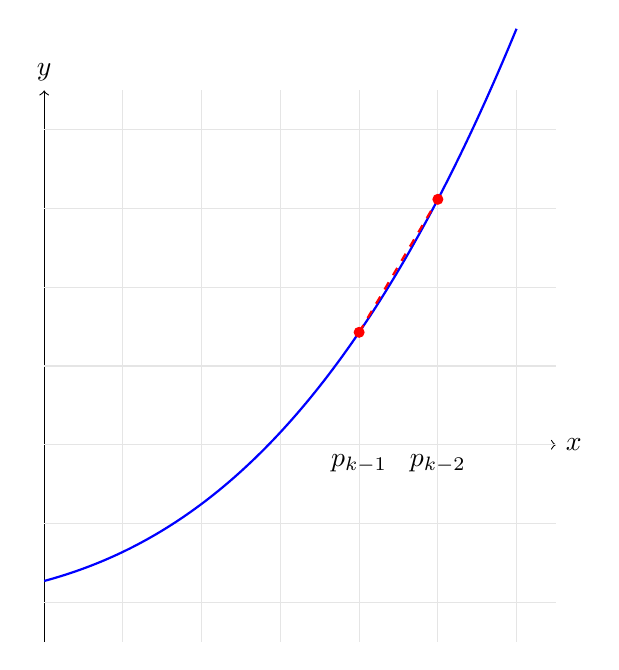
\begin{tikzpicture}[scale=1]
  % Axes
    \draw[->] (0,0) -- (6.5,0) node[right] {$x$};
    \draw[->] (0,-2.5) -- (0,4.5) node[above] {$y$};

  % Grid
    \foreach \x in {1,...,6} {
      \draw[gray!20] (\x,-2.5) -- (\x,4.5);
    }
    \foreach \y in {-2,-1,0,1,2,3,4} {
      \draw[gray!20] (0,\y) -- (6.5,\y);
    }

  % Labels for xticks
    \node[below] at (4,0) {$p_{k-1}$};
    \node[below] at (5,0) {$p_{k-2}$};

  % Function plot
    \draw[blue, thick, domain=0:6, samples=100, smooth, variable=\x] 
      plot ({\x}, {0.01*(\x + 3)^3 - 2});

  % Points
    \pgfmathsetmacro{\yA}{0.01*(4+3)^3 - 2} % = 0.01 * 343 - 2 = 3.43 - 2 = 1.43
    \pgfmathsetmacro{\yB}{0.01*(5+3)^3 - 2} % = 0.01 * 512 - 2 = 5.12 - 2 = 3.12
    \fill[red] (4,\yA) circle (2pt);
    \fill[red] (5,\yB) circle (2pt);

  % Secant line: from (4, \yA) to (5, \yB)
    \draw[red, dashed, thick] 
      (4,\yA) -- (5,\yB);

  % Optional: label the line
  % \node[anchor=south, red] at (4.5,{(\yA+\yB)/2}) 
  %   {\small $y = \frac{\yB - \yA}{1} (x - 4) + \yA$};

  \end{tikzpicture}
\end{center}

both newton's method and the secant method have the limitation that they may
diverge when the initial guess is not sufficiently close to the root. In 
bisection, we used the idea of bracketing the root at each step to ensure
convergence. 

\section{False Position}

If instead of considering a midpoint approximation for the root \newline
($\displaystyle p_k \approx p_0 + \frac{p_1 - p_0}{2}$), we consider a
secant approximation for the root (based on the endpoints of the interval).
This is called the \textbf{Method of False Position}.

\[
p_k \approx p_1 - f(p_1) \frac{p_1-p_0}{f(p_0)-f(p_1)}
.\]

\section{oops, skipped a bunch of pages}

\section{Error Analysis}

We want to be able to give a more precise description of how a method converges
to a the solution. For example, consider finding a root for the polynomial

\[
x^3 + 4x^2 - 10 = 0
.\]

with two different methods (A and B). Suppose that the errors produced by these 
methods are as given below.

\begin{table}[h]
    \centering
    \begin{tabular}{|c|c|c|}
        \hline
        & \textbf{Method A} & \textbf{Method B} \\
        \hline
        $|p - p_0|$ & 0.134769987 & 0.134769987 \\
        $|p - p_1|$ & 0.078276245 & 0.008103332 \\
        $|p - p_2|$ & 0.037310791 & 0.000003811 \\
        $|p - p_3|$ & 0.019771639 & 0.000000000 \\
        $|p - p_4|$ & 0.009940240 & \text{to all significant digits} \\
        \hline
    \end{tabular}
    \caption{Comparison of Methods A and B}
\end{table}

Notice that the error for method $A$ decreases by a constant factor (about 2)
at each iteration. For method $B$, the error drops off much more quickly. The
error at step $n$ is roughly proportional to the error at step $n-1$, squared.

\textbf{Both of these behaviours can be quantified.}

\noindent\defn Suppose $\{ p_n \}_{n=0}^\infty$ is a sequence that converges to $p$,
with $p_n \neq p$ for all $n$. If positive constants $\lambda$ and $\alpha$
exist with $\displaystyle \lim_{n\to\infty} \frac{|p_{n+1}-p|}{|p_n -p|^\alpha} = \lambda$
then $\{ p_n \}_{n=0}^\infty$ converges to $p$ of order $\alpha$, with asymptotic
error constant $\lambda$.

Notice that:
\begin{itemize}
\item a sequence with high order of convergence converges more rapidly than a
  sequence with a lower order.
\item the constant $\lambda$ affects the speed of convergence, but is not as
  important as the order ($\alpha$).
\item We want a large $\alpha$. $\alpha \geq 1$ is sufficient. \\
  If $\alpha = 0.5$, for example, then the error at $k$ is proportional
  to the square root of the error at $k-1$. This is not a good behaviour.
\end{itemize}

\subsection{Common Cases}

For different values of $\alpha$, we observe the following convergence behaviors:

\begin{itemize}
    \item $\alpha = 1$, $\lambda < 1$: Linearly convergent.
    \[ \bigEps_{n+1} \approx \lambda \bigEps_n \]
    
    \item $\alpha = 2$: Quadratically convergent.
    \[ \bigEps_{n+1} \approx \lambda \bigEps_n^2 \]
    
    \item $\alpha$ does not have to be an integer. For example, the secant method has:
    \[ \alpha = \frac{1+\sqrt{5}}{2} < 2. \]
\end{itemize}

\textbf{In order to truly understand the behaviour of a method, we need to
  find both the order and the asymptotic error constant.}

\section{Thm (2.7 of Text)}

Let $g\in C[a,b]$ s.t. $g(x) \in [a, b]$ for all $x \in [a, b]$.

Suppose, in addition, that $g'$ is continuous on $(a,b)$ and a constant
$0\leq k<1$ exists with $|g'(x)|\leq k$ for all $x\in (a,b)$.

If $g'(p) \neq 0$, then for any number $p_0$ in $[a,b]$ the sequence 

\[
  p_n = g(p_{n-1}) \text{ for } n\geq 1
.\]

converges only linearly to the unique fixed point $p$ in $[a,b]$.

\proof We know from the fixed point theorem that the sequence converges to $p$.
since $g'$ exists on $[a,b]$ we can apply the mean value theorem to g:

\[
\underbrace{g(p_n) - g(p)}_{p_{n+1} - p} = g'(\xi_n)(p_n - p)
.\]

where $\xi_n$ is between $p_n$ and $p$. Thus,

\[
  \frac{p_{n+1}-p}{p_n-p} = g'(\xi_n)
.\]

and fixed point iteration gives linear convergence with asymptotic error
constant $|g'(p)|$ whenever $g'(p) \neq 0$.


\section{Thm (2.7 of Text)}

Let $g\in C[a,b]$ s.t. $g(x) \in [a, b]$ for all $x \in [a, b]$.

Suppose, in addition, that $g'$ is continuous on $(a,b)$ and a constant
$0\leq k<1$ exists with $|g'(x)|\leq k$ for all $x\in (a,b)$.

If $g'(p) \neq 0$, then for any number $p_0$ in $[a,b]$ the sequence 

\[
  p_n = g(p_{n-1}) \text{ for } n\geq 1
.\]

converges only linearly to the unique fixed point $p$ in $[a,b]$.

\proof We know from the fixed point theorem that the sequence converges to $p$.
since $g'$ exists on $[a,b]$ we can apply the mean value theorem to g:

\[
\underbrace{g(p_n) - g(p)}_{p_{n+1} - p} = g'(\xi_n)(p_n - p)
.\]

where $\xi_n$ is between $p_n$ and $p$. Thus,

\[
  \frac{p_{n+1}-p}{p_n-p} = g'(\xi_n)
.\]

and fixed point iteration gives linear convergence with asymptotic error
constant $|g'(p)|$ whenever $g'(p) \neq 0$.

\proof...

Thus $\displaystyle \lim_{n\to\infty} \frac{|p_{n+1}-p|}{|p_n-p|} = |g'(p)|$
and fixed-point iteration gives linear convergence with asymptotic error 
constant $|g'(p)|$ whenever $g'(p) \neq 0$.

Method $A$ was the fixed-point iteration method defined by the iteration
function

\[
  g(x) = \frac{1}{2} (10-x^3)^{1/2}
.\]

Notice that:

\begin{align*}
g'(p=1.365230013)
&= -\frac{3}{4}x^2(10-x^3)^{-1/2} \\
&= -0.51 \neq 0
\end{align*}

so the theorem applies if we consider the interval $[1, 1.5]$ and we see that
linear convergence is obtained. On the other hand, Method $B$ was the fixed
point iteration method defined by the iteration function

\[
g(x) = x-\frac{x^3+4x^2-10}{3x^2+8x}
.\]

This method gave quadratic convergence, but the theorem cannot be applied 
because

\[
g'(p) = 0
.\]

We saw last day that higher order convergence for fixed point method can 
occur only when $g'(p) = 0$. It is possible under certain reasonable conditions
to obtain quadratic convergence...

\section{Theorem (2.8 of Text)}

Let $p$ be a solution of the equation $x = g(x)$.

Suppose $g'(p) = 0$ and $g''$ is continuous and strictly bounded by $M$ on an
open interval $I$ containing $p$. Then, there exists a $\delta > 0$ such that
for $p_0 \in [p-\delta, p+\delta]$, the sequence defined by $p_n = g(p_{n-1})$
when $n\geq 1$ converges at least quadratically to $p$.

Moreover, for sufficiently large values of $n$, 

\[
|p_{n+1} - p| < \frac{M}{2} |p_n - p|^2
.\]

\proof... (see lecture notes)

Thus the sequence $\{ p_n \}_{n=0}^\infty$ converges quadratically if
$g''(p) \neq 0$ and higher order convergent if $g''(p) = 0$. Also, we know
$|g''| < M $ so 

\[
|p_{n+1} - p| < \frac{M}{2} |p_n - p|^2
.\]

So the idea behind finding iteration methods with a high order of convergence
is to look for schemes whose derivatives are zero at the fixed point.

\section{Newton's Method}

\begin{align*}
  g(x) &= x-\frac{f(x)}{f'(x)} \\
  g'(x) &= 1-\frac{[f'(x)]^2 - f(x) f''(x)}{[f'(x)]^2} \\
        &= \frac{f(x)f''(x)}{[f'(x)]^2} \\
\end{align*}

$\therefore g'(p) = 0$ provided $f'(p) \neq 0$.

$\therefore$ Newton's Method satisfies the derivative condition for \thm 2.8.

\pagebreak

Let's take another look at Newton's Method. Consider using Newton's Method to
find the roots of

\[
p^3 - p^3 - p + 1 = 0
.\]

Newton's Method here is

\[
  p_{n+1} = p_n = \frac{p_n^3 - p_n^2 - p_n + 1}{3p_n^2 - 2p_n -1}
.\]

Starting from $p_0 = 1.1$ we find

\begin{table}[h]
  \centering
  \begin{tabular}{c|c}
    \textbf{Iteration} & \textbf{Value} \\
    \hline
    $p_0$ & 1.1 \\
    $p_1$ & 1.05116\ldots \\
    $p_2$ & 1.02589\ldots \\
    $p_3$ & 1.01303\ldots \\
    $p_4$ & 1.00653\ldots \\
    $p_5$ & 1.00327\ldots \\
    \vdots & \vdots
  \end{tabular}
  \caption{Numerical Iterations}
  \label{tab:iterations}
\end{table}

Which is very slow (Linear) convergence to the root (which is $p=1$).

Why is this?

In Newton's Method, we need to find $f'(p) \neq 0 $ to obtaine quadratic 
convergence. Notice that

\[
  f'(p) = 3p^2 - 2p - 1 |_{p=1} = 0
.\]

So the theorem doesn't hold. Moreover, factoring $f$:

\[
f(x) = (x-1)^2(x+1)
.\]

we see that $x=1$ is a zero with multiplicity of $2$.

\defn A solution $p$ of $f(x) = 0$ is a zero of multiplicity $m$ of $f$ if for 
$x\ne p$ we can write $f(x) = (x-p)^m q(x)$ where $\lim_{x\to p} q(x) \neq 0$.

Simple zeros are those that have multiplicity $1$.

Thus Newton's Method can only be applied to simple zeros of a function.
Identification fo the multiplicity of a zero is often made easier by the two
following theorems.

\thm 2.10

$f\in C'[a,b]$ has a simple zero at $p$ in $(a,b)$ if and only if $f(p) = 0$
but $f'(p) \neq 0$.

\thm 2.11

The function $f\in C^m[a,b]$ has a zero of multiplicity $m$ at $p$ if and only
if 

\[
  0 = f(p) = f'(p) = f''(p) = \dots = f^{(m-1)}(p)
.\]

but $f^{(m)}(p) \neq 0$.

We want to obtain quadratic convergence with Newton's Method for multiple roots.

One approach is to define a new function

\[
  \mu(x) = f\frac{(x)}{f'(x)}
.\]

We assume $p$ is a zero of multiplicity $m$ and $f(x) = (x-p)^m q(x)$ where
$q(p) \neq 0$. Then,

\begin{align*}
  \mu(x) &= \frac{(x-p)^m}{m(x-p)^{m-1} q(x) + q'(x)(x-p)^m} \\
  &= \frac{(x-p)q(x)}{mq(x) + q'(x) (x-p)}  \\
  &= (x-p) \frac{q(x)}{mq(x)+q'(x-p)} \\
  q(p) \neq 0 \quad\text{therefore, } &\mu(p) \text{ has a simple root at } x=p
\end{align*}

so $\mu(p) = 0$, but $\displaystyle \frac{q(p)}{mq(p) + q'(p)(p-p)} = \frac{1}{m} \neq 0$.
and $p$ is a zero of multiplicity $1$ of $\mu(x)$.

\textbf{Good:}
\begin{itemize}
  \item Quadratic convergence for all roots
\end{itemize}

\textbf{Bad:}
\begin{itemize}
  \item Need $f''$
  \item $\mu$ is more expensive to work with
  \item $\mu$ might give more roundoff error
\end{itemize}



\include{cleaned/Lecture019} % chapter 3 supposed to start here

\chapter{Approximation and Interpolation}
\begin{greenquote}
  Chapter 3 of the textbook.
\end{greenquote}

This is the section about splines! You are going to love splines.

\section{Approximation and Interpolation}

It is often useful or necessary to approximate a complicated or expensive function,
or a function only known at a discrete set of points, by a smpler function
which can be computed or evaluated more easily over a whole interval. When the
function in question is known accurately at a discrete set of points, we are
inclined to use an interpolation procedure- where the graph of the approximating 
function runs exactly through the points of the discrete set. 

If the dataset is expected to contain error, which is the case for measurements
or observations in experimental studies, a better strategy is to allow the
graph of the approximating function to stray from the data points.

% insert image here

A useful and well known class of functions for mapping the set of real numbers
into itself is the class of algebraic polynomials.

\[
  P_n(x) = a_nx^n + a_{n-1}x^{n-1} + \dots + a_1x + a_0
.\]

where $n$ is a non-negative integer and $a_i$ are real constants. Polynomials 
have the desirable property that they can approximate \uline{any} function
over a closed, bounded interval.

This desired property is precisely captured by the \textbf{Weierstrass 
Approximation Theorem}

\pagebreak

\subsection{The Weierstrass Approximation Theorem}

Suppose $f \in C[a,b]$. 

$\forall \bigEps > 0 \exists P \in \{ \mathbb{P}_n , C[a,b] \}$ such that

\[
  |f(x)-P(x)| < \epsilon \forall x \in [a,b]
.\]

\begin{figure}[h]
    \centering
    \resizebox{0.8\textwidth}{!}{%
        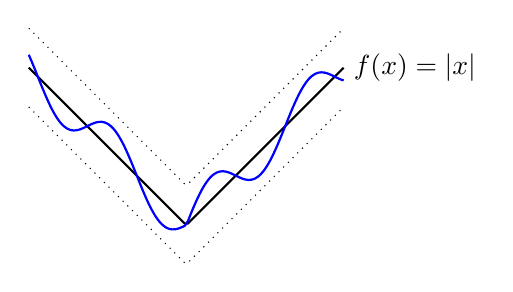
\begin{tikzpicture}
            % Define the function
            \draw[thick] plot[samples=100,domain=-2:2] (\x,{abs(\x)}) node[right] {$f(x) = |x|$};

            % Epsilon bounds
            \draw[dotted] plot[samples=100,domain=-2:2] (\x,{abs(\x) + 0.5});
            \draw[dotted] plot[samples=100,domain=-2:2] (\x,{abs(\x) - 0.5});

            % Labeling epsilon
            % \draw[->] (1,1.5) -- (1.1,1.2) node[midway,right] {$\varepsilon$};
            % \draw[->] (-1,1.5) -- (-1.1,1.2) node[midway,left] {$\varepsilon$};

            % Approximation function (squiggly)
            \draw[thick,blue] plot[smooth, samples=100, domain=-2:2] (\x, {0.3*sin(5*\x r) + abs(\x)});

        \end{tikzpicture}%
    }
    \caption{Polynomial approximation to $f(x) = |x|$.}
\end{figure}

This is a very strong theorem, as it only requires $f(x)$ to be continuous on 
the interval, and not necessarily differentiable.

Unfortunately, the Weierstrass Approximation Theorem does not tell us how to 
select such a polynomial. Many would immediately jump to using Taylor series
polynomials for polynomial interpolation, however, Taylor series' concentrate
their accuracy at the point $a$ rather than over the entire interval, and are
typically poorly suited for interpolation.

\subsubsection{Taylor Series Polynomials}

\[
P_n(x) = f(a) + f'(a)(x-a) + \frac{f''(a)}{2!}(x-a)^2 + \dots + \frac{f^{(n)}(a)}{n!}(x-a)^n
.\]

A particularly clear demonstration of this drawback is seen for

\[
f(x) = \frac{1}{x} \qquad \text{expanded about } x_0 = 1
.\]

Then,

\begin{align*}
  P_n(x) &= \sum_{k=0}^n \frac{f^{(k)}(1)}{k!}(x-1)^k\\
         &= \sum_{k=0}^n (-1)^k(x-1)^k \\
\end{align*}

To approximate $f(3)=\frac{1}{3}$ by $P_n(3)$ for increasing values of $n$, we
see a dramatic and catastrophic failure: 

\begin{table}[h]
    \centering
    \renewcommand{\arraystretch}{1.4}
    \begin{tabular}{|c|c|c|c|c|c|c|c|c|}
        \hline
        \( n \) & 0 & 1 & 2 & 3 & 4 & 5 & 6 & 7 \\ 
        \hline
        \( P_n(3) \) & 1 & -1 & 3 & -5 & 11 & -21 & 43 & -85 \\ 
        \hline
    \end{tabular}
    \caption{Values of \( P_n(3) \) for increasing \( n \).}
\end{table}

We will insetad focus on methods which use information throughout the entire 
interval to approximate $f$.

\section{Polynomial Interpolation}

We now assume that the given dataset is exact and represents values of some
unknown function. We want to find the polynomial $P_n(x)$ of the smallest 
possible degree $n$ such that

\[
P_n(x_k) = f_k \qquad k = 1,2, \dots, N
.\]

for $N+1$ distinct interpolation points $x_0,\dots,x_N$ and $N+1$ values 
$\underbrace{f_0,\dots,f_N}_{\text{data points}}$.

To solve this problem, we will first investigate the simpler problem where all
the data equals zero, except at one point.

We are looking for a polynomial $L_m(x)$ of degree $\leq N$ such that

\[
  L_m(x_k) = \delta_{mk} \qquad = \begin{cases}
    1 & k = m \\
    0 & k \neq m
    \end{cases}
.\]


\begin{center}

\begin{tikzpicture}[overlay, remember picture]
    \draw[thick,->] (0,0) node[below]{\textbf{Kronecker Delta}} to (-1.1,0.8);
\end{tikzpicture}
\end{center}

This is easy to find. Since the polynomial must vanish at the points 
$x_k, k\neq m$, it must contain the factors

\[
  (x-x_k) \qquad \text{for } k \neq m
.\]

\[
\therefore L_m(x) = c \cdot \prod_{k=0; k\neq m}^N(x-x_k)
.\]

The constant is determined by the condition $L_m(x_m) = 1$.

\[
\implies L_m(x) = \prod_{k=0; k\neq m}^{N}  \frac{x-x_k}{x_m-x_k}
.\]

Typically, 
\begin{center}
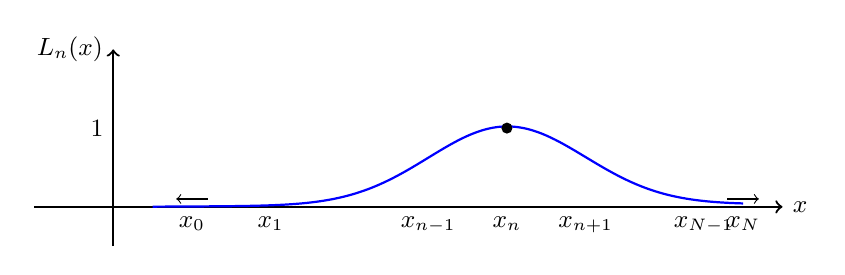
\begin{tikzpicture}
    % Axes
    \draw[thick,->] (-1,0) -- (8.5,0) node[right] {\small $x$}; % x-axis
    \draw[thick,->] (0,-0.5) -- (0,2) node[left] {\small $L_n(x)$}; % y-axis

    % Labels on axes
    \node[left] at (0,1) {\small 1}; % Label at y = 1

    % Points on x-axis
    \foreach \x/\label in {1/$x_0$, 2/$x_1$, 4/$x_{n-1}$, 5/$x_n$, 6/$x_{n+1}$, 7.5/$x_{N-1}$, 8/$x_N$}
        \node[below] at (\x,0) {\small \label};

    % Sinusoidal-like Lagrange basis function
    \draw[thick,blue,domain=0.5:8,samples=100,smooth] 
        plot (\x, {exp(-0.5*(\x-5)^2) * cos(2*pi*(\x-5)/3) + 0.05*sin(5*\x)});

    % Highlight peak at x_n
    \fill (5,1) circle (2pt);
    
    % Small arrows at edges
    \draw[->] (7.8,0.1) -- (8.2,0.1);
    \draw[->] (1.2,0.1) -- (0.8,0.1);
    
\end{tikzpicture}
\end{center}

These polynomials are the building blocks for deriving a polynomial
interpolating a general function. It is easy to see that

\[
  P(x) = \sum_{m=0}^N f_m < L_m(x)
.\]

is a polynomial of degree $\leq N$ satisfying the interpolation conditions.

This polynomial is called the $n^{th}$ \textbf{Lagrange Interpolating Polynomial} 

Recall that we wanted to find the polynomial $P_n(x)$ of smallest degree such
that 

\[
  P_n(x_k) = f_k \qquad k = 0,\dots,N
.\]

\subsection{Uniqueness}

Is this polynomial unique?

\textbf{Yes.} 

\proof Assume there are two different polynomials $p$ and $q$ of degree $\leq N$
which both satisfy the interpolation conditions. Their difference, $d=p-q$, is
also a polynomial of degree $\leq N$ and vanishes at the $N+1$ distinct points 
$x_0,\dots,x_N$.

However, a nonzero polynomial of degree $\leq N$ has at most $N$ zeros, this

\[
d = p-q = 0 \implies \begin{cases}
  p=q\\
  \text{ uniqueness}
\end{cases}
\]

$\therefore$ the $n^{th}$ Lagrange Interpolating Polynomial is the unique
interpolating polynomial satisfying the interpolation conditions.

\subsection{Example}

Fit a cubic through the first four points of the table 

\begin{table}[h]
    \centering
    \begin{tabular}{c|c|c}
        $i$ & $x^i$ & $f(x_i)$ \\
        \hline
        0 & 3.2 & 22.0 \\
        1 & 2.7 & 17.8 \\
        2 & 1.0 & 14.2 \\
        3 & 4.8 & 38.3 \\
        4 & 5.6 & 51.7 \\
    \end{tabular}
    % \caption{Tabular representation of given data}
    % \label{tab:data}
\end{table}

and use it to find the interpolated value for $x=3.0$.

\soln The $3^{rd}$ Lagrange Interpolating Polynomial is given by

\begin{align*}
    P(x) = &\ \frac{(x - x_1)(x - x_2)(x - x_3)}{(x_0 - x_1)(x_0 - x_2)(x_0 - x_3)} f_0 \\
    &+ \frac{(x - x_0)(x - x_2)(x - x_3)}{(x_1 - x_0)(x_1 - x_2)(x_1 - x_3)} f_1 \\
    &+ \frac{(x - x_0)(x - x_1)(x - x_3)}{(x_2 - x_0)(x_2 - x_1)(x_2 - x_3)} f_2 \\
    &+ \frac{(x - x_0)(x - x_1)(x - x_2)}{(x_3 - x_0)(x_3 - x_1)(x_3 - x_2)} f_3
\end{align*}

Substituting the values from the table and evaluating at $x=3.0$ gives 

\begin{align*}
    P(3.0) = &\ \frac{(3.0 - 2.7)(3.0 - 1.0)(3.0 - 4.8)}{(3.2 - 2.7)(3.2 - 1.0)(3.2 - 4.8)} (22.0) \\
    &+ \frac{(3.0 - 3.2)(3.0 - 1.0)(3.0 - 4.8)}{(2.7 - 3.2)(2.7 - 1.0)(2.7 - 4.8)} (17.8) \\
    &+ \frac{(3.0 - 3.2)(3.0 - 2.7)(3.0 - 4.8)}{(1.0 - 3.2)(1.0 - 2.7)(1.0 - 4.8)} (14.2) \\
    &+ \frac{(3.0 - 3.2)(3.0 - 2.7)(3.0 - 1.0)}{(4.8 - 3.2)(4.8 - 2.7)(4.8 - 1.0)} (38.3) \\
    &= 20.21
\end{align*}

Our next task is to develop estimates for the error. As it turns out, the form
of the error (but not necessarily the magnitude) resembles that of the $n^{th}$
Taylor Polynomial.

\subsection{Error Estimates}

*The lecture ended just before this section*

\thm (3.3 of Text)

Suppose $x_0, \dots, x_n$ are distinct numbers in the interval $[a,b]$ and
$f\in C^{n+1}[a,b]$. Then for each $x\in [a,b]$, a number $\xi(x)\in(a,b)$
exists with the property

\[
  f(x) = P(x) + \frac{f^{(n+1)}(\xi(x))}{(n+1)!} (x-x_0) (x-x_1) \dots (x-x_n)
.\]

\begin{center}

\begin{tikzpicture}[overlay, remember picture]
    \draw[thick,->] (-2,0) node[below]{\textbf{n-th Langrange Interpolating Polynomial}} to (-3.2,0.6);
\end{tikzpicture}
\end{center}

*do you guys like my diagrams with arrows?*


\section{Continued from Lecture 20}

Our next task is to develop estimates for the error. As it turns out, the form
of the error (but not necessarily the magnitude) resembles that of the $n^{th}$
Taylor Polynomial.

\subsection{Error Estimates}

\thm (3.3 of Text)

Suppose $x_0, \dots, x_n$ are distinct numbers in the interval $[a,b]$ and
$f\in C^{n+1}[a,b]$. Then for each $x\in [a,b]$, a number $\xi(x)\in(a,b)$
exists with the property

\[
  f(x) = P(x) + \frac{f^{(n+1)}(\xi(x))}{(n+1)!} (x-x_0) (x-x_1) \dots (x-x_n)
.\]

\begin{center}

\begin{tikzpicture}[overlay, remember picture]
    \draw[thick,->] (-2,0) node[below]{\textbf{n-th Langrange Interpolating Polynomial}} to (-3.2,0.6);
\end{tikzpicture}
\end{center}

Recall: If $f$ has $(n+1)$ continuous derivatives on $[a,b]$ and $P(x)$ is the 
interpolating polynomial of degree $\leq n$ for $f$ at the points 
$x_0, \dots, x_n$, then,

\[
  f(x) - P(x) = \frac{f^{(n+1)}(\xi (x))}{(n+1)!} \prod_{k=0}^{n} (x-x_k)
.\]

\Ex suppose you need to construct six-decimal-place tables for the common, or
base-10, logarithm function from $x=1$ to $x=10$ in a way that linear 
interpolation is accurate within $10^{-6}$ of the true value. Determine a bound
for the step size for this table.

Based on the following data:

\begin{table}[h]
    \centering
    \begin{tabular}{c c c}
        \toprule
        $i$ & $x_i$ & $f(x_i)$ \\
        \midrule
        0 & 3.2 & 22.0 \\
        1 & 2.7 & 17.8 \\
        2 & 1.0 & 14.2 \\
        3 & 4.8 & 38.3 \\
        4 & 5.6 & 51.7 \\
        \bottomrule
    \end{tabular}
    % \caption{Tabulated data of $x_i$ and $f(x_i)$ values}
    % \label{tab:data}
\end{table}

find approximations to $f(3)$ using the $2^{nd}$ and $3^{rd}$ Lagrange
interpolating polynomials.

\soln we will use $x_0, x_1$ and $x_3$ to build the $2^{nd}$ Lagrange
interpreting polynomial.

\begin{align*}
P_2(3) &= \frac{(3 - 2.7)(3 - 4.8)}{(3.2 - 2.7)(3.2 - 4.8)} (22.0) \\
&\quad + \frac{(3 - 3.2)(3 - 4.8)}{(2.7 - 3.2)(2.7 - 4.8)} (17.8) \\
&\quad + \frac{(3 - 3.2)(3 - 2.7)}{(4.8 - 3.2)(4.8 - 2.7)} (38.3) \\
&\approx 20.27
\end{align*}

We will use $x_0, x_1, x_2, x_3$ to build the $3^{rd}$ Lagrange
interpolating polynomial.

\begin{align*}
P_3(3) &= \frac{(3.0 - 2.7)(3.0 - 1.0)(3.0 - 4.8)}{(3.2 - 2.7)(3.2 - 1.0)(3.2 - 4.8)} (22.0) \\
&\quad + \frac{(3.0 - 3.2)(3.0 - 1.0)(3.0 - 4.8)}{(2.7 - 3.2)(2.7 - 1.0)(2.7 - 4.8)} (17.8) \\
&\quad + \frac{(3.0 - 3.2)(3.0 - 2.7)(3.0 - 4.8)}{(1.0 - 3.2)(1.0 - 2.7)(1.0 - 4.8)} (14.2) \\
&\quad + \frac{(3.0 - 3.2)(3.0 - 2.7)(3.0 - 1.0)}{(4.8 - 3.2)(4.8 - 2.7)(4.8 - 1.0)} (38.3) \\
&\approx 20.21
\end{align*}

Notice that:

\begin{enumerate}
\item We do not know the derivative values of $f$, therefore we cannot apply 
  the error formula. However, we can make an estimate for the error by examining
  polynomials of different degrees by using different nodes.

\item The $P_2$-calculation was not used to reduce the work in calculating $P_3$.
  We want to find a way to use previous degrees of $P$, especially since the 
  previous point implies that we will examine the results for Lagrange 
  polynomials of varying degrees.
\end{enumerate}

\noindent
We want to examine polynomials based on different nodes. In the last example, 
we considered the polynomial based on the nodes $x_0, x_1 \text{ and } x_3$

We will call this polyomial $\mathbf{P_{013}(x)}$

\noindent
We also considered the polynomial based on the nodes $x_0, x_1, x_2, x_3$

We will call this polyomial $\mathbf{P_{0123}(x)}$

Similarly, we make the following definition:

Let $f$ be a function defined at $x_0, x_1, x_2, \dots, x_n$ and suppose that
$m_1, m_2, \dots ,m_k$ are $k$ distinct integers with $0\leq m_i \leq n$ and
for each $i$. 

The Lagrange Interpolating Polynomial that agrees with $f$ at 
$x_m, x_{m2}, \dots, x_{mk}$ is denoted

\[
  P_{m_1, m_2, \dots, m_k}
.\]

Using this notation,

\[
P_0(x) = f(x_0)
\]

\[
P_1(x) = \frac{(x - x_1) f(x_0) + (x - x_0) f(x_1)}{x_0 - x_1}
\]

and 


\begin{align*}
  P_{0,1}(x) &= \left( \frac{x - x_1}{x_0 - x_1} \right) f(x_0) + \left( \frac{x - x_0}{x_1 - x_0} \right) f(x_1) \\
             &= \frac{(x - x_1) P_0(x) - (x - x_0) P_1(x)}{x_0 - x_1}
\end{align*}

So $P_{0,1}(x)$ can be recursively defined in terms of $P_0(x)$ and $P_1(x)$.

More generally:

\thm Let $f$ be defined at $x_0, x_1, \dots, x_k$ and $x_j$ and $x_i$ be two
distinct numbers in this set. Then

\[
  P_{0,1,\dots,k}(x) = 
  \frac{(x - x_j) P_{0,1,\dots,j,j+1,\dots,n}(x) - (x - x_i) P_{0,1,\dots,i-1,i+1,\dots,n}(x)}{x_i - x_j}
.\]

\proof I left out the proof.

The corresponding procedure is called Neville's Method. Here, values for each 
interpolating polynomial are generated using previous calculations.

\Ex $\displaystyle P_{0,1}(x) = \frac{(x-x_1)P_0 - (x-x_0) P_1}{(x_0 - x_1)}$ is
derived from $P_0 + P_1$. Correspondingly, $P_{1,2}(x)$ is derived from $P_1$
and $P_2$.

Written as a table:

\begin{figure}[h]
    \centering
    \includegraphics[width=0.8\textwidth]{./assets/Lecture 021 Neville's Method Table.jpg}
\end{figure}

\Ex suppose $x_j = j$ for $j=0,1,2,3$ and it is known that 

\begin{align*}
  &P_{0,1}(x) = 2x+1 \\
  &P_{0,2}(x) = x+1 \\
  &P_{1,2,3}(2.5) = 3
\end{align*}

Find $P_{0123}(2.5)$.

We have $P_{123}$ and we need another quadratic to find our $P_{0123}$

\[
P_{0,1,2} = \frac{(x-x_1)P_{02} (x) - (x-x_2) P_{01}(x)}{x_2 - x_1}
.\]

We evaluate $P_{02}(2.5) = 2.25$ and $P_{01}(2.5) = 6$

We have $x_1 = 1, x_2 = 2, x=2.5$

\[
  P_{012}(2.5) = 2.25 
.\]

\[
  P_{0123}(2.5) = \frac{(2.25-x_0)P_{123}(2.25) - (2.25-x_3)P_{012}(2.25)}{x_3 -
  x_0} = 2.875
\]


\include{cleaned/Lecture022}
\include{cleaned/Lecture023}
Even if we enforce the constraint that $f$ and $f'$ agree at the nodes, we still
have the problem that $P_n$ will be expensive to compute for large $n$ and that
for high $n$, the interpolating polynomial can still oscillate wildly.

\section{Splines (15.1)}

Previously, we used a single polynomial to compute an approximation to a
function over some finite interval. We increased the degree of the polynomial if
we wanted more accuracy. However, increasing the degree of the polynomial causes
oscillatory behaviour, and high degree polynomials have the property that a
fluctuation over a small portion of the interval can induce large fluctuations
over the entire interval.

An alternative approach is to divide the interval into subintervals and use a
different, lower degree polynomial in each subinterval. These polynomials are
patched together to give a piecewise polynomial approximation. 

\subsection{Possible Choices}
 
\subsubsection{Piecewise Linear Interpolation}

We join a set of data points by a series of straight lines.

The biggest disadvantage of this approach is that the approximation is typically
not smooth. \ie it is not differentiable at these points, which may not be
satisfactory.

\subsubsection{Piecewise Polynomails of Hermite Type}

*Hermite is pronounced \enquote{her-meat}

If we know the value of a function \textbf{and} it's derivative at each of the
data points, then we could use a Hermite cubic polynomial on each interval
$[x_i, x_{i+1}]$ to approximate the function. Often, however, the derivative of
the function is not known at the data points.

\subsubsection{Piecewise Quadratic Polynomials}

Alternatively, we could join a set of polynomials with quadratic polynomials.
This gives us $3$ arbitrary constants. There will be $2$ conditions to fit the
curve through the endpoints of each interval, but there isn't enough flexibility
to set conditions on the derivative at both endpoints $x$ and $x_n$.

We have enough flexibility to set conditions for the first $n-1$ data points,
but the data point $x_n$ requires four conditions, when we can only provide
three degrees of freedom.

\begin{itemize}
\item $P_0$: 2 endpoint conditions + 1 slope condition
\item $P_1$: 2 endpoint conditions + 1 slope conditions
\item $P_n$: 2 endpoint conditions + 2 slope conditions
\end{itemize}

\subsubsection{Cubic Spline Interpolation}

If we use cubic polynomials between each successive pair of nodes, then there
are four constants and it is possible to ensure that the interpolant

\begin{itemize}
  \item agrees with the function at all the nodes
  \item is continuously differentiable
  \item has continuous second derivatives
\end{itemize}

Given a function $f$ defined on $[a, b]$ and a set of nodes
$a=x_0<x_1<\dots<x_n=b$, a cubic spline interpolant $S$ for $f$ is a function
that satisfies the following:

\begin{itemize}
  \item $S(x) = S_j(x)$ on $[x_j, x_{j+1}]$
  \item $S_j(x_{j+1}) = f(x_{j+1}) = S_{j+1}(x_j)$ splines must pass through the
    data points
  \item $S_j'(x_{j+1}) = S'_{j+1}(x_{j+1})$ first derivative is continuous
  \item $S_j''(x_{j+1}) = S''_{j+1}(x_{j+1})$ second derivative is continuous
\end{itemize}

We also need a boundary condition. Typically one of the following hold in the
problems we will consider: 

\begin{itemize}
  \item $S'(x_0) = f'(x_0)$ and $S'(x_n) = f'(x_n)$ 
    \enquote{Clamped Boundary Conditions}
  \item $S''(x_0) = 0 = S''(x_n)$
    \enquote{Free or Natural Boundary Conditions} \\
    \small{
    *Natural Boundary Conditions tell us that $S$ is not curved at the endpoints.
  }
\end{itemize}

Of course, for the clamped case, we need derivative information, either from the
physics or from some assumption. If there are $(n+1)$ points, the number of
intervals and the number of $S_i(x)$'s are $n:$

\[
  S_i(x) = a_i + b_i (x-x_i) + c_i (x-x_i)^2 + d_i (x-x_i)^3
.\]

Letting $h_i = x_{i+1} - x_i$  we can simplify by substituting $x_{i+1}$ and
$x_i$ into $S_i(x)$, $S_i'(x)$ and $S_i''(x)$. Eliminating the $b_i$ and $d_i$
gives a linear system of equations:

\begin{align*}
&h_{i-1}c_{i-1} + 2(h_{i-1} + h_i)c_i + h_0 c_{i+1} \\
&\quad= \frac{3}{h_i}(a_{i+1}-a_i) - \frac{3}{h_{i-1}}(a_i - a_{i-1})\\
&\quad 1 \leq i \leq n-1
\end{align*}

where the $a_i$ are known

\[
  a_i = f(x_i) \qquad 0 \leq i \leq n-1
.\]

and we define 

\begin{align*}
  a_n &\equiv f(x_n) \\
  b_n &\equiv f'(x_n) \\
  c_n &\equiv \frac{f''(x_n)}{2}
\end{align*}

The $b_i$ and $d_i$ are easily found:

\[
  b_i = \frac{1}{h_i}(a_{i+1} - a_i) - \frac{h_i}{3} (2c_i + c_{i+1}) \quad 0 \leq i \leq n-1
.\]

\[
  d_i = \frac{c_{i+1} - c_i}{3h_i}
.\]

We still need to impose the boundary conditions:

\textbf{Natural Boundary Conditions}
Consider the Natural BC's: $S''(x_0) = S''(x_n) = 0$.

\[
\therefore C_n = 0 \quad\text{(by definition)}
.\]

\[
S_0''(x) = 2C_0 + 6d_0(x-x_0) \therefore S''(x_0) = 2c_0 + 6d_0(x_0-x_0) = 0 =
c_0
.\]

We can derive a matrix equation for the $[c_i]$:

\[
Ax = b
.\]

where 

\[
  A = \begin{bmatrix}
    1 & 0 & 0 & \dots & \dots &  0 \\
    h_0 & 2(h_0+h_1) & h_1 & \ddots & &  \vdots\\
    0 & h_1 & 2(h_1+h_2) & h_2 & \ddots  & \vdots\\
    \vdots & & \ddots & \ddots & \ddots  & \vdots\\
    \vdots & & & h_{n-2} & 2(h_{n-2}+h_{n-1}) & h_{n-1}  \\
    0 & \dots & \dots & 0 & 0 & 1
  \end{bmatrix}
\]

\[
 x=\begin{bmatrix}
 c_0\\
 c_1\\
 \vdots\\
 c_n\\
 \end{bmatrix}
.\]

\[
b=\begin{bmatrix}
0\\
\frac{3}{h_1}(a_2-a_1)-\frac{3}{h_0}(a_1-a_0)\\
\vdots\\
\frac{3}{h_{n-1}}(a_{n}-a_{n-l})-\frac{3}{h_{n-2}}(a_{n-1}-a_{n-2})\\
0
\end{bmatrix}
.\]

There exists a unique solution for the $c_i$'s.

The matrix is strictly diagonally dominant, so it is invertible and a unique
solution for the $c_i$ exists.

First we need a definition and a theorem.

\defn The $n \times n$ matrix $A$ is strictily diagonally dominant if 

\[
  |a_{ii}| > \sum_{j=1; j\neq i}^{n} |a_{ij}|
.\]

holds for each $i = 1, \dots, n$.

\thm A strictly diagonally dominant matrix is invertible.

Also note that the matrix $A$ is \textbf{tridiagonal}: all entires are zero
except for a band which is 3 entries wide centred on the main diagonal.

Solutions to tridiagonal linear systems can be found very efficiently:

*Only O(n) operations are needed using methods we shall discuss later

\textbf{Clamped Boundary Conditions}
We also want to treat clamped boundary conditions:

\[
f'(a) = S'(a) = S_0'(x_0) = b_0 + 2c_0 (x_0-x_0) + 3d_0 (x_0-x_0)^2 = b_0
.\]

but 
\[
  b_{i-1} = \frac{a_i - a_{i-1}}{h_{i-1}} - \frac{h_{i-1}}{3}(2c_{i-1} + c_i)
.\]

\[
\therefore b_0 = \frac{a_1 - a_0}{h_0} - \frac{h_0}{3}(2c_0 + c_1)
.\]

\[
\implies 2h_0c_0 + h_0 c_1 = \frac{3}{h_0}(a_1 - a_0) - 3f'(a)
.\]

Similarly, 

\[
  h_{n-1} c_{n-1} + 2h_{n-1} c_n = 3f'(b) - \frac{3}{h_{n-1}}(a_{n-1} - a_n)
.\]

Once again, we obtain a strictly diagonally dominant linear system

\begin{center}
  $\implies$ A unique solution exists for the $c_i$'s
\end{center}

Furthermore, the system is tridiagonal so it can be solved efficiently for the
coefficients of the spline.



\chapter{Numerical Differentiation}
\begin{greenquote}
  Chapter 4 of the textbook. This section is also about Numerical Integration,
  Richardson's Extrapolation, Romberg Integration, Adaptive Quadrature and
  Gaussian Quadrature.
\end{greenquote}

\include{cleaned/Lecture025}
\include{cleaned/Lecture026}
\include{cleaned/Lecture027}
\include{cleaned/Lecture028}
\include{cleaned/Lecture029}
\include{cleaned/Lecture030}
\section{Initial Value Problems for ordinary Differential Equations}

Many natural, scientific and engineering problems can be described in terms of 
\uline{differential equations}. Differential equations give us a way to
mathematically expres rates of change. We will be considering methods for
treating ordinary differential equations (ODEs) in this lecture. ODEs only
consider derivatives with respect to one variable.

\Ex Let $y(t)$ denote the number of individuals in a certain population. If this
population has a constant growth rate $\alpha$ (the difference between a
constant birth rate and death rate), then the differential equation 

\[
y'(t) = \alpha y(t)
.\]

with initial condition $y(0) = y_0$ describes the population growth.

\soln 

% \begin{align*}
%   \frac{y'}{y} &= \alpha \\
%   \frac{dy}{y} &= \alpha \, dx \\
%   \int \frac{dy}{y} &= \int \alpha \, dx \\
%   \ln |y| &= \alpha x + C \\
%   |y| &= e^{\alpha x + C} = e^C \cdot e^{\alpha x} \\
%   y &= C_1 e^{\alpha x} \quad \text{where } C_1 = \pm e^C
% \end{align*}

\begin{align*}
  \frac{y'(t)}{y(t)} &= \alpha \\
  D_t[\ln(y(t))] &= \alpha \\
  \ln(y(t)) &= \alpha t + \text{const}  \\
  y(t) &= ce^{\alpha t} \qquad c = e^{\text{const}}\\
\end{align*}

\begin{equation*}
  y(0) = y_0 \implies y(t) = y_0 e^{\alpha t}
.\end{equation*}

To include other effects such as overcrowding, competition for food, etc, one
might introduce a second term into the equation

\begin{equation*}
  y'(t) = \alpha y(t) - \beta [y(t)]^2
.\end{equation*}

where $\beta > 0$ and $\beta$ is small. Introducing a nonlinear term makes the
problem much more difficult to study analytically.

Indeed, few problems originating from the study of physical phenomena can be
solved exactly. We begin by studying numerical methods for approximating the
solution $y(t)$ to a problem.

\[
  \frac{dy}{dt} = f(t, y) \qquad \text{for } a \leq t \leq b
.\]

subject to the initial condition 

\[
y(a) = \alpha
.\]

\subsection{The elementary theory of initial value problems}

We want/need some theoretical results, in particular, we would like to show that
solutions to equations exist and are unique.

\defn A function $f(t,y)$ satisfies a Lipschitz condition in the variable $y$ on
a set $D \in \mathbb{R}^2$ if a constant $L > 0$ exists such that

\[
  |f(t,y_1) - f(t, y_2)| \leq L|y_1 - y_2| \qquad \text{for all } (t,y_1), (t,y_2) \in D
.\]

The constant $L$ is called a \uline{Lipschitz constant} for $f$.

\pagebreak
\subsubsection{Example}

Does $f(t,y) = ty$ satisfy a Lipschitz condition on 

\[
D  = \{(t,y) : 0 \leq t \leq 1, -\infty < y < \infty\}
?\]

\noindent
\soln

% \begin{align*}
% &|f(t,y_1) - f(t, y_2)| \\
% &= |-ty_1 + \frac{4t}{y_1} + ty_2 - \frac{4t}{y_2}|\\
% \end{align*}

\begin{equation*}
|f(t,y_1) - f(t, y_2)| = |-ty_1 + \frac{4t}{y_1} + ty_2 - \frac{4t}{y_2}|
.\end{equation*}


Consider $y_1 = -1, t=1$, $y_2 \to 0^+$. Under these conditions, we have
$|f(t,y_1) - f(t,y_2)| \to \infty$.

RHS = $L|y_1-y_2| \to L$

$L$ is finite.

We cannot have $|f(t,y_1) - f(t,y_2)| \leq L|y_1 - y_2|$ for any finite $L$

$\therefore$ Lipschitz condition does not hold.


IDK why but he starts off with this example

\section{Quadrature Formula Example}

Find the constants $c_0, c_i$ and $x$ such that the quadrature formula

\begin{equation*}
  \int_{-1}^{0} f(x) \, dx = c_0 f(-1) + c_i f(x_1)
.\end{equation*}

has the highest degree of precision possible.

\uline{ans.}
 
\renewcommand{\arraystretch}{3}
\begin{center}
  \begin{tabular}{c|c}
    Function $f$ & Equation \\
    \hline
    $f(x) = 1$ & $\displaystyle \int_{-1}^{0} 1 \, dx = c_0 + c_i$ \\
    $f(x) = x$ & $\displaystyle \int_{-1}^{0} x \, dx = \left. \frac{x^2}{2} \right|_{-1}^0 = c_0 (-1) + c_i x_1 = -\frac{1}{2}$ \\
    $f(x) = x^2$ & $\displaystyle \int_{-1}^{0} x^2 \, dx = c_0 + c_i x_1^2 = \frac{1}{3}$ \\
  \end{tabular}
\end{center}

Next, we do some substutitions:

\begin{enumerate}
\item substitute (1) into (2) to eliminate $c_0$
\item substitute (1) into (3) to eliminate $c_0$
\end{enumerate}

We now have $2$ equations for $c_i + x_1$.

Solve: $c_0 = \frac{1}{4}, c_i = \frac{3}{4}, x_i = -\frac{1}{3}$

Could it be exact for cubics?

LHS = $\int_{-1}^{0} x^3 \, dx = -\frac{1}{4}$

RHS = $-\underbrace{c_0}_{\frac{1}{4}} +
\underbrace{c_i}_{\frac{3}{4}}\underbrace{x_i}_{-\frac{1}{3}}^3 \neq \text{LHS} $

So, no, it cannot be exact for cubics.

\section{Legendre Polynomials}

This approach can be used to obtain the nodes and coefficients for larger $n$,
but Legendre polynomials can be used to obtain them more easily.

The Legendre Polynomials are defined according to the following two properties:

\begin{enumerate}
\item $P_n(x)$ is a polynomial of degree $n$.\\
  $\implies P_0(x) = 1$ 
\item $\int_{-1}^{1} P(x)P_n(x) \, dx = 0$ whenever $P(x)$ is a polynomial of
  degree less than $n$.
\end{enumerate}

The first few Legendre polynomials are

\renewcommand{\arraystretch}{1.25}
\begin{center}
  \begin{tabular}{c|c}
    $P_n(x)$ & \\ \hline
    $P_0(x)$ & $1$ \\
    $P_1(x)$ & $x$ \\
    $P_2(x)$ & $x^2-\frac{1}{3}$ \\
    $P_3(x)$ & $x^3-\frac{3}{5}x$ \\
    $P_4(x)$ & $x^4-\frac{6}{7}x^2+\frac{3}{35}$ \\
  \end{tabular}
\end{center}

Some properties:

\begin{itemize}
\item The roots of these polynomials are distinct
\item The roots of these polynomials lie in $(-1, 1)$
\item The $P_n$'s are symmetrical about the origin\\
  $\implies$ the roots are symmetrical about the origin
\item The roots of the $n^{th}$ degree Legendre polynomial have the property
  that they are the nodes needed to produce an integral approximation formula
  that gives the exact result for any polynomial of degree less than $2n$.
\end{itemize}

\thm Suppose $x_1, x_2, \dots, x_n$ are the roots of the $n^{th}$ degree
Legendre polynomial $P_n(x)$ and that for each $i=1, 2, \dots, n$ the numbers
$c_i$ are defined by

\begin{equation*}
  c_i = \int_{-1}^{1} \prod_{\substack{j = 1 \\ j \ne i}}^{n} \frac{x-x_j}{x_i-x_j} \, dx
.\end{equation*}

If $P(x)$ is any polynomial of degree less than $2n$ then

\begin{equation*}
  \int_{-1}^{1} P(x) \, dx = \sum_{i=1}^{n} c_i P(x_i)
.\end{equation*}


\include{cleaned/Lecture032}
\section{Euler's Method}
This section starts with Euler's Method Error Analysis. The analysis is
straightforward, and interesting because it can be extended to the higher order
methods that will be discussed in later sections. To derive the proof of
convergence, we need the following

\lemma: If $s$ and $t$ are positive real numbers, $\{a_i\}_{i=0}^k$ is a
sequence satisfying
\begin{align*}
  a_0 &\geq -\frac{t}{s} \\
  a_{i+1} &\leq (1+s) a_i + t \quad i = 0, 1, \ldots, k
\end{align*}
then $\displaystyle a_{i+1}\leq e^{(i+1)s}\left(a_0 + \frac{t}{s}\right) - \frac{t}{s}$

The proof of the lemme is not important, but it is included in section 23.5 of
the Chapter 5 lecture notes.

\subsection{Theorem 1 (23.6)}
Suppose $f$ is continuous and satisifes a Lipschitz condition with constant $L$
on
\[
D = \{(t,y) : a \leq t \leq b, -\infty < y < \infty \}
.\]
and that a constant $M$ exists with the property that
\[
  \abs{y''(t)} \leq M
.\]
Let $y(t)$ denote the unique solution to the initial value problem
\[
  y' = f(t,y); \quad y(a) = y_0, a \leq t \leq b
.\]
and $w_0, w_1, \dots, w_N$ be the approximations generated by Euler's Method.

Then, for each $i=0, \dots, N$, 
\[
  \abs{y(t_i) - w_i} \leq \frac{hM}{2L}\left[e^{L(t_i-a)}-1\right]
.\]

\proof (23.7) (I didn't add it yet)

Note that the theorem \uline{requires} that  
\[
  \abs{y''(t)} \leq M
.\]
The second derivative $y''(t)$ may not be known, but if $\frac{\partial
f}{\partial t}$ and $\frac{\partial f}{\partial y}$ exist,
\begin{align*}
  y''(t) = \frac{d}{dt} y'(t) &= \frac{df}{dt}(t,y(t)) \\
                              &= \frac{\partial f}{\partial
  t}(t,y(t)) + \frac{\partial f}{\partial y}(t,y(t)) \cdot f(t,y(t))
\end{align*}

\subsubsection{Example (23.8)}
What value of $h$ is needed to ensure that $\abs{y(t_i) - w_i} \leq 0.1$ for the
initial value problem
\[
  \begin{cases}
    y' = \frac{2}{t} y + t^2 e^t & 1 \leq t \leq 2 \\
    y = 0 & t = 1
  .\end{cases}
.\]
You are given $y''(t) = (2+4t+t^2)e^t - 2e$

\soln (23.9) $y''(t)$ is increasing and positive on $[1,2]$, so
\begin{align*}
  \abs{y''(t)} &\leq \abs{y''(2)} \\
  &= 14e^2 - 2e \\
  &= 98.0102 \\
\end{align*}
\begin{align*}
  \text{since}\quad & \abs{\frac{\partial}{\partial y} \left(\frac{2}{t}y +
  t^2e^2\right)} \\
                &\quad\leq \abs{\frac{2}{t}} \\
                &\quad\leq 2 \\
\end{align*}
a Lipschitz Constant for $f(t,y) = \frac{2}{t}y+t^2e^t$ is $L = 2$.
\[
\therefore \abs{y(t_i) - w_i} \leq \frac{hM}{2L}\left[e^{L(t_i-1)}-1\right] \leq
0.1
.\]
we need to choose $h$ so that $\displaystyle \frac{98.0102h}{4}
\left[e^{2(2-1)}-1 \right] \leq 0.1$.
\[
\implies h \leq \frac{0.4}{98.0102(e^2-1)} = 0.00064
.\]

\section{The Difference Method}
We ned a way to compare the efficiency of different approximation methods. The
difference method compares how much the exact solution to the differential
equation fails to satisfy the difference equation being used for the approximation.

\defn The Difference Method
\begin{align*}
  w_0 &= \alpha \\
  w_{i+1} &= w_i + h \phi (t_i, w_i)
\end{align*}
has a local trunctation error 
\begin{align*}
  \tau_{i+1}(h) &= \frac{y(t_{i+1}) - (y(t_i) + h \phi (t_i, y(t_i)))}{h} \\
                &= \frac{y(t_{i+1}) - y(t_i)}{h} - \phi(t_i, y(t_i)) 
                & i = 0, 1, \dots, N-1
\end{align*}

\subsection{Example: Euler's Method (23.11)}
The difference method for Euler's Method has $\phi = f$.
\begin{align*}
  w_0 &= \alpha \\
  w_{i+1} &= w_i + h \phi(t_i, w_i) = w_i + h f(t_i, w_i)
\end{align*}
has local truncation error
\begin{align*}
  \tau_{i+1}(h) &= \frac{y(t_{i+1}) - y(t_i)}{h} - f(t_i, y(t_i)) \\
                &= \frac{y(t_i) + hy'(t_i) + \frac{h^2}{2}y''(\xi)}{den} & \text{we do a taylor expansion} \\
\end{align*}

Local truncation errors are called local because they measure hte accuracy of
the method at a specific step, assuming the method was exact at the previous
steps. We obviously want the local truncation error to be small. Often, methods
for solving ODE's are derived so that the local truncation errors are of the
form
\[
O(h^p)
.\]
for the largest possible $p$, while keeping the number of operations reasonable.

\subsection{How to obtain improved accuracy?}
\ie a larger $p$ in the $O(h^p)$ local truncation error.

Suppose we want to approximate the solution to the ivp 
\[
  \begin{cases}
    y' = f(t,y) & a \leq t \leq b\\
    y = \alpha & t = 0
  .\end{cases}
.\]
where $y(t) \in C^{(n+1)} [a,b]$

One approach is to expand the solution in terms of its $n^{th}$ Taylor
Polynomial about $t_i$.
\begin{align*}
	y(t_{i+1}) &= y(t_i) + h y'(t_i) + \frac{h^2}{2} y''(t_i) + \cdots + \frac{h^n}{n!} y^{(n)}(t_i) + R \\
		   &= y(t_i) + h f\pqty{t_i, y(t_i)} + \frac{h^2}{2} f'\pqty{t_i, y(t_i)} + \cdots + \frac{h^n}{n!} f^{(n-1)}\pqty{t_i, y(t_i)} + R \\
  \text{where} \quad R &= \frac{h^{n+1}}{(n+1)!} y^{(n+1)}\pqty{\xi_i}
\end{align*}

\section{The Taylor Method of Order $n$}
If we drop the remainder term, we obtain the \textbf{Taylor Method of Order $n$}.
\begin{align*}
  \begin{cases}
    w_0 = \alpha & \\
    w_{i+1} = w_i + hT^{(n)}(t_i, w_i) & i = 0, 1, \dots, N-1
  .\end{cases}
\end{align*}
where $T^{(n)}(t_i, w_i) = f(t_i, w_i) + \frac{h}{2}f'(t_i, w_i) + \dots + 
\frac{h^n}{n!}f^{(n)}(t_i, w_i)$ is the $n^{th}$ Taylor Polynomial of $f$ about
$t_i$.

Note: \textit{Euler's Method is equivalent to Taylor's Method of Order $1$}.


\include{cleaned/Lecture034}
\section{Higher order Runge-Kutta Methods (24.8)}
Third order Runge-Kutta methods are not commonly used. However, fourth order
Runge-Kutta methods are widely used and derived in a similar fashion. Greater
complexity results from having to compare terms through $h^4$ and this gives a
set of 11 equations in 13 unknowns. The set of equations can be solved with 2
unknowns being chosen arbitrarily. 

The most commonly used set of values leads to the following algorithm:
\begin{align*}
  w_{n+1} &= w_n+\frac{1}{6}\bqty{k_1+2k_2+2k_3+k_4} \\
  k_1 &= hf(t_n, w_n) \\
  k_2 &= hf\bqty{t_n+\frac{1}{2}h, w_n + \frac{1}{2}k_1} \\
  k_3 &= hf\bqty{t_n+\frac{1}{2}h, w_n + \frac{1}{2}k_2} \\
  k_4 &= hf\bqty{t_n+h, w_n + k_3}
\end{align*}

The main computational effort in applying Runge-Kutta methods is the evaluation
of $f$. In the second order methods, the local truncation error is $\order{h^2}$
and the cost is two functional evaluations per step. The Runge-Kutta method of
order four requires four evaluations per step and the local truncation error is
$\order{h^4}$.

We may wonder about higher order formulas\dots

\subsection{Error Analysis of Higher Order Runge-Kutta Methods (24.9)}
Butcher has shown that the following relationship holds:

\begin{tabular}{c|ccccccc}
  evaluations & $2$ & $3$ & $4$ & $5\leq n\leq7$ & $8\leq n\leq9$ & $10\leq n$\\
  Best LTE & $O(h^2)$ & $O(h^3)$ & $O(h^4)$ & $O(h^{n-1})$ &
  $O(h^{n-2})$ &$O(h^{n-3})$
\end{tabular}

This indicates why methods of order $\leq 5$ are often used rather than higher
order methods with a larger step size.



\end{document}
